\documentclass{article}
\usepackage[final]{neurips_2025}  % NEURIPS style (neurips_2025.sty is in paper_draft/)
\usepackage[hidelinks]{hyperref}  % REQUIRED: clickable links
\usepackage{booktabs}  % REQUIRED: professional tables
\usepackage{graphicx}
\usepackage{amsmath,amssymb}

% The style file only defines the footer track name when a track option is given;
% define the main-track text here so that the mandated [final] option compiles.
\makeatletter
\providecommand{\@trackname}{\@neuripsordinal\ Conference on Neural Information Processing Systems (NeurIPS \@neuripsyear).}
\makeatother

% Additional packages
\usepackage[utf8]{inputenc}
\usepackage[T1]{fontenc}
\usepackage{multirow}
\usepackage{enumitem}
\usepackage{algorithm}
\usepackage[noend]{algpseudocode}
\usepackage{tikz}
\usetikzlibrary{arrows.meta,positioning}

% Import command files
%%%%% MATH NOTATION MACROS %%%%%
% Standard math notation for academic papers
% Import with: %%%%% MATH NOTATION MACROS %%%%%
% Standard math notation for academic papers
% Import with: %%%%% MATH NOTATION MACROS %%%%%
% Standard math notation for academic papers
% Import with: \input{commands/math}

\usepackage{amsmath,amsfonts,bm}

%%%%%%%%%%%%%%%%%%%%%%%%%%%%%%%%%%%%%%%%%%%%%%%%%%%%%%%%%%%%%%%%%
% FIGURE AND SECTION REFERENCES
%%%%%%%%%%%%%%%%%%%%%%%%%%%%%%%%%%%%%%%%%%%%%%%%%%%%%%%%%%%%%%%%%

% Mark sections of captions for referring to divisions of figures
\newcommand{\figleft}{{\em (Left)}}
\newcommand{\figcenter}{{\em (Center)}}
\newcommand{\figright}{{\em (Right)}}
\newcommand{\figtop}{{\em (Top)}}
\newcommand{\figbottom}{{\em (Bottom)}}
\newcommand{\captiona}{{\em (a)}}
\newcommand{\captionb}{{\em (b)}}
\newcommand{\captionc}{{\em (c)}}
\newcommand{\captiond}{{\em (d)}}

% Figure references
\def\figref#1{figure~\ref{#1}}
\def\Figref#1{Figure~\ref{#1}}
\def\twofigref#1#2{figures \ref{#1} and \ref{#2}}
\def\quadfigref#1#2#3#4{figures \ref{#1}, \ref{#2}, \ref{#3} and \ref{#4}}

% Section references
\def\secref#1{section~\ref{#1}}
\def\Secref#1{Section~\ref{#1}}
\def\twosecrefs#1#2{sections \ref{#1} and \ref{#2}}
\def\secrefs#1#2#3{sections \ref{#1}, \ref{#2} and \ref{#3}}

% Equation references
\def\eqref#1{equation~\ref{#1}}
\def\Eqref#1{Equation~\ref{#1}}
\def\plaineqref#1{\ref{#1}}

% Algorithm references
\def\algref#1{algorithm~\ref{#1}}
\def\Algref#1{Algorithm~\ref{#1}}
\def\twoalgref#1#2{algorithms \ref{#1} and \ref{#2}}
\def\Twoalgref#1#2{Algorithms \ref{#1} and \ref{#2}}

% Table references
\def\tabref#1{table~\ref{#1}}
\def\Tabref#1{Table~\ref{#1}}

% Chapter references
\def\chapref#1{chapter~\ref{#1}}
\def\Chapref#1{Chapter~\ref{#1}}

%%%%%%%%%%%%%%%%%%%%%%%%%%%%%%%%%%%%%%%%%%%%%%%%%%%%%%%%%%%%%%%%%
% BASIC MATH DEFINITIONS
%%%%%%%%%%%%%%%%%%%%%%%%%%%%%%%%%%%%%%%%%%%%%%%%%%%%%%%%%%%%%%%%%

\def\ceil#1{\lceil #1 \rceil}
\def\floor#1{\lfloor #1 \rfloor}
\def\1{\bm{1}}
\def\eps{{\epsilon}}

% Common operators
\DeclareMathOperator*{\argmax}{arg\,max}
\DeclareMathOperator*{\argmin}{arg\,min}
\DeclareMathOperator{\sign}{sign}
\DeclareMathOperator{\Tr}{Tr}
\let\ab\allowbreak

%%%%%%%%%%%%%%%%%%%%%%%%%%%%%%%%%%%%%%%%%%%%%%%%%%%%%%%%%%%%%%%%%
% VECTORS (lowercase bold)
%%%%%%%%%%%%%%%%%%%%%%%%%%%%%%%%%%%%%%%%%%%%%%%%%%%%%%%%%%%%%%%%%

\def\vzero{{\bm{0}}}
\def\vone{{\bm{1}}}
\def\vmu{{\bm{\mu}}}
\def\vtheta{{\bm{\theta}}}
\def\va{{\bm{a}}}
\def\vb{{\bm{b}}}
\def\vc{{\bm{c}}}
\def\vd{{\bm{d}}}
\def\ve{{\bm{e}}}
\def\vf{{\bm{f}}}
\def\vg{{\bm{g}}}
\def\vh{{\bm{h}}}
\def\vi{{\bm{i}}}
\def\vj{{\bm{j}}}
\def\vk{{\bm{k}}}
\def\vl{{\bm{l}}}
\def\vm{{\bm{m}}}
\def\vn{{\bm{n}}}
\def\vo{{\bm{o}}}
\def\vp{{\bm{p}}}
\def\vq{{\bm{q}}}
\def\vr{{\bm{r}}}
\def\vs{{\bm{s}}}
\def\vt{{\bm{t}}}
\def\vu{{\bm{u}}}
\def\vv{{\bm{v}}}
\def\vw{{\bm{w}}}
\def\vx{{\bm{x}}}
\def\vy{{\bm{y}}}
\def\vz{{\bm{z}}}

%%%%%%%%%%%%%%%%%%%%%%%%%%%%%%%%%%%%%%%%%%%%%%%%%%%%%%%%%%%%%%%%%
% MATRICES (uppercase bold)
%%%%%%%%%%%%%%%%%%%%%%%%%%%%%%%%%%%%%%%%%%%%%%%%%%%%%%%%%%%%%%%%%

\def\mA{{\bm{A}}}
\def\mB{{\bm{B}}}
\def\mC{{\bm{C}}}
\def\mD{{\bm{D}}}
\def\mE{{\bm{E}}}
\def\mF{{\bm{F}}}
\def\mG{{\bm{G}}}
\def\mH{{\bm{H}}}
\def\mI{{\bm{I}}}
\def\mJ{{\bm{J}}}
\def\mK{{\bm{K}}}
\def\mL{{\bm{L}}}
\def\mM{{\bm{M}}}
\def\mN{{\bm{N}}}
\def\mO{{\bm{O}}}
\def\mP{{\bm{P}}}
\def\mQ{{\bm{Q}}}
\def\mR{{\bm{R}}}
\def\mS{{\bm{S}}}
\def\mT{{\bm{T}}}
\def\mU{{\bm{U}}}
\def\mV{{\bm{V}}}
\def\mW{{\bm{W}}}
\def\mX{{\bm{X}}}
\def\mY{{\bm{Y}}}
\def\mZ{{\bm{Z}}}
\def\mBeta{{\bm{\beta}}}
\def\mPhi{{\bm{\Phi}}}
\def\mLambda{{\bm{\Lambda}}}
\def\mSigma{{\bm{\Sigma}}}

%%%%%%%%%%%%%%%%%%%%%%%%%%%%%%%%%%%%%%%%%%%%%%%%%%%%%%%%%%%%%%%%%
% CALLIGRAPHIC (mathcal)
%%%%%%%%%%%%%%%%%%%%%%%%%%%%%%%%%%%%%%%%%%%%%%%%%%%%%%%%%%%%%%%%%

\def\gA{{\mathcal{A}}}
\def\gB{{\mathcal{B}}}
\def\gC{{\mathcal{C}}}
\def\gD{{\mathcal{D}}}
\def\gE{{\mathcal{E}}}
\def\gF{{\mathcal{F}}}
\def\gG{{\mathcal{G}}}
\def\gH{{\mathcal{H}}}
\def\gI{{\mathcal{I}}}
\def\gJ{{\mathcal{J}}}
\def\gK{{\mathcal{K}}}
\def\gL{{\mathcal{L}}}
\def\gM{{\mathcal{M}}}
\def\gN{{\mathcal{N}}}
\def\gO{{\mathcal{O}}}
\def\gP{{\mathcal{P}}}
\def\gQ{{\mathcal{Q}}}
\def\gR{{\mathcal{R}}}
\def\gS{{\mathcal{S}}}
\def\gT{{\mathcal{T}}}
\def\gU{{\mathcal{U}}}
\def\gV{{\mathcal{V}}}
\def\gW{{\mathcal{W}}}
\def\gX{{\mathcal{X}}}
\def\gY{{\mathcal{Y}}}
\def\gZ{{\mathcal{Z}}}

%%%%%%%%%%%%%%%%%%%%%%%%%%%%%%%%%%%%%%%%%%%%%%%%%%%%%%%%%%%%%%%%%
% SETS (blackboard bold)
%%%%%%%%%%%%%%%%%%%%%%%%%%%%%%%%%%%%%%%%%%%%%%%%%%%%%%%%%%%%%%%%%

\def\sA{{\mathbb{A}}}
\def\sB{{\mathbb{B}}}
\def\sC{{\mathbb{C}}}
\def\sD{{\mathbb{D}}}
\def\sF{{\mathbb{F}}}
\def\sG{{\mathbb{G}}}
\def\sH{{\mathbb{H}}}
\def\sI{{\mathbb{I}}}
\def\sJ{{\mathbb{J}}}
\def\sK{{\mathbb{K}}}
\def\sL{{\mathbb{L}}}
\def\sM{{\mathbb{M}}}
\def\sN{{\mathbb{N}}}
\def\sO{{\mathbb{O}}}
\def\sP{{\mathbb{P}}}
\def\sQ{{\mathbb{Q}}}
\def\sR{{\mathbb{R}}}
\def\sS{{\mathbb{S}}}
\def\sT{{\mathbb{T}}}
\def\sU{{\mathbb{U}}}
\def\sV{{\mathbb{V}}}
\def\sW{{\mathbb{W}}}
\def\sX{{\mathbb{X}}}
\def\sY{{\mathbb{Y}}}
\def\sZ{{\mathbb{Z}}}

%%%%%%%%%%%%%%%%%%%%%%%%%%%%%%%%%%%%%%%%%%%%%%%%%%%%%%%%%%%%%%%%%
% COMMON MATH SHORTCUTS
%%%%%%%%%%%%%%%%%%%%%%%%%%%%%%%%%%%%%%%%%%%%%%%%%%%%%%%%%%%%%%%%%

% Expectation and variance
\newcommand{\E}{\mathbb{E}}
\newcommand{\Var}{\mathrm{Var}}
\newcommand{\Cov}{\mathrm{Cov}}
\newcommand{\R}{\mathbb{R}}

% Datasets
\newcommand{\train}{\mathcal{D}}
\newcommand{\valid}{\mathcal{D_{\mathrm{valid}}}}
\newcommand{\test}{\mathcal{D_{\mathrm{test}}}}

% Distributions
\newcommand{\laplace}{\mathrm{Laplace}}
\newcommand{\Uniform}{\mathrm{Unif}}
\newcommand{\Normal}{\mathrm{Normal}}
\newcommand{\Categorical}{\mathrm{Categorical}}

% Common functions
\newcommand{\softmax}{\mathrm{softmax}}
\newcommand{\sigmoid}{\sigma}
\newcommand{\KL}{D_{\mathrm{KL}}}

% Norms
\newcommand{\normlzero}{L^0}
\newcommand{\normlone}{L^1}
\newcommand{\normltwo}{L^2}
\newcommand{\normlp}{L^p}
\newcommand{\normmax}{L^\infty}

%%%%%%%%%%%%%%%%%%%%%%%%%%%%%%%%%%%%%%%%%%%%%%%%%%%%%%%%%%%%%%%%%
% DEFINITIONS AND HIGHLIGHTING
%%%%%%%%%%%%%%%%%%%%%%%%%%%%%%%%%%%%%%%%%%%%%%%%%%%%%%%%%%%%%%%%%

% Highlight a newly defined term
\newcommand{\newterm}[1]{{\bf #1}}
\newcommand{\defn}[1]{\textbf{#1}}
\newcommand{\defeq}{\mathrel{\stackrel{\textnormal{\tiny def}}{=}}}


\usepackage{amsmath,amsfonts,bm}

%%%%%%%%%%%%%%%%%%%%%%%%%%%%%%%%%%%%%%%%%%%%%%%%%%%%%%%%%%%%%%%%%
% FIGURE AND SECTION REFERENCES
%%%%%%%%%%%%%%%%%%%%%%%%%%%%%%%%%%%%%%%%%%%%%%%%%%%%%%%%%%%%%%%%%

% Mark sections of captions for referring to divisions of figures
\newcommand{\figleft}{{\em (Left)}}
\newcommand{\figcenter}{{\em (Center)}}
\newcommand{\figright}{{\em (Right)}}
\newcommand{\figtop}{{\em (Top)}}
\newcommand{\figbottom}{{\em (Bottom)}}
\newcommand{\captiona}{{\em (a)}}
\newcommand{\captionb}{{\em (b)}}
\newcommand{\captionc}{{\em (c)}}
\newcommand{\captiond}{{\em (d)}}

% Figure references
\def\figref#1{figure~\ref{#1}}
\def\Figref#1{Figure~\ref{#1}}
\def\twofigref#1#2{figures \ref{#1} and \ref{#2}}
\def\quadfigref#1#2#3#4{figures \ref{#1}, \ref{#2}, \ref{#3} and \ref{#4}}

% Section references
\def\secref#1{section~\ref{#1}}
\def\Secref#1{Section~\ref{#1}}
\def\twosecrefs#1#2{sections \ref{#1} and \ref{#2}}
\def\secrefs#1#2#3{sections \ref{#1}, \ref{#2} and \ref{#3}}

% Equation references
\def\eqref#1{equation~\ref{#1}}
\def\Eqref#1{Equation~\ref{#1}}
\def\plaineqref#1{\ref{#1}}

% Algorithm references
\def\algref#1{algorithm~\ref{#1}}
\def\Algref#1{Algorithm~\ref{#1}}
\def\twoalgref#1#2{algorithms \ref{#1} and \ref{#2}}
\def\Twoalgref#1#2{Algorithms \ref{#1} and \ref{#2}}

% Table references
\def\tabref#1{table~\ref{#1}}
\def\Tabref#1{Table~\ref{#1}}

% Chapter references
\def\chapref#1{chapter~\ref{#1}}
\def\Chapref#1{Chapter~\ref{#1}}

%%%%%%%%%%%%%%%%%%%%%%%%%%%%%%%%%%%%%%%%%%%%%%%%%%%%%%%%%%%%%%%%%
% BASIC MATH DEFINITIONS
%%%%%%%%%%%%%%%%%%%%%%%%%%%%%%%%%%%%%%%%%%%%%%%%%%%%%%%%%%%%%%%%%

\def\ceil#1{\lceil #1 \rceil}
\def\floor#1{\lfloor #1 \rfloor}
\def\1{\bm{1}}
\def\eps{{\epsilon}}

% Common operators
\DeclareMathOperator*{\argmax}{arg\,max}
\DeclareMathOperator*{\argmin}{arg\,min}
\DeclareMathOperator{\sign}{sign}
\DeclareMathOperator{\Tr}{Tr}
\let\ab\allowbreak

%%%%%%%%%%%%%%%%%%%%%%%%%%%%%%%%%%%%%%%%%%%%%%%%%%%%%%%%%%%%%%%%%
% VECTORS (lowercase bold)
%%%%%%%%%%%%%%%%%%%%%%%%%%%%%%%%%%%%%%%%%%%%%%%%%%%%%%%%%%%%%%%%%

\def\vzero{{\bm{0}}}
\def\vone{{\bm{1}}}
\def\vmu{{\bm{\mu}}}
\def\vtheta{{\bm{\theta}}}
\def\va{{\bm{a}}}
\def\vb{{\bm{b}}}
\def\vc{{\bm{c}}}
\def\vd{{\bm{d}}}
\def\ve{{\bm{e}}}
\def\vf{{\bm{f}}}
\def\vg{{\bm{g}}}
\def\vh{{\bm{h}}}
\def\vi{{\bm{i}}}
\def\vj{{\bm{j}}}
\def\vk{{\bm{k}}}
\def\vl{{\bm{l}}}
\def\vm{{\bm{m}}}
\def\vn{{\bm{n}}}
\def\vo{{\bm{o}}}
\def\vp{{\bm{p}}}
\def\vq{{\bm{q}}}
\def\vr{{\bm{r}}}
\def\vs{{\bm{s}}}
\def\vt{{\bm{t}}}
\def\vu{{\bm{u}}}
\def\vv{{\bm{v}}}
\def\vw{{\bm{w}}}
\def\vx{{\bm{x}}}
\def\vy{{\bm{y}}}
\def\vz{{\bm{z}}}

%%%%%%%%%%%%%%%%%%%%%%%%%%%%%%%%%%%%%%%%%%%%%%%%%%%%%%%%%%%%%%%%%
% MATRICES (uppercase bold)
%%%%%%%%%%%%%%%%%%%%%%%%%%%%%%%%%%%%%%%%%%%%%%%%%%%%%%%%%%%%%%%%%

\def\mA{{\bm{A}}}
\def\mB{{\bm{B}}}
\def\mC{{\bm{C}}}
\def\mD{{\bm{D}}}
\def\mE{{\bm{E}}}
\def\mF{{\bm{F}}}
\def\mG{{\bm{G}}}
\def\mH{{\bm{H}}}
\def\mI{{\bm{I}}}
\def\mJ{{\bm{J}}}
\def\mK{{\bm{K}}}
\def\mL{{\bm{L}}}
\def\mM{{\bm{M}}}
\def\mN{{\bm{N}}}
\def\mO{{\bm{O}}}
\def\mP{{\bm{P}}}
\def\mQ{{\bm{Q}}}
\def\mR{{\bm{R}}}
\def\mS{{\bm{S}}}
\def\mT{{\bm{T}}}
\def\mU{{\bm{U}}}
\def\mV{{\bm{V}}}
\def\mW{{\bm{W}}}
\def\mX{{\bm{X}}}
\def\mY{{\bm{Y}}}
\def\mZ{{\bm{Z}}}
\def\mBeta{{\bm{\beta}}}
\def\mPhi{{\bm{\Phi}}}
\def\mLambda{{\bm{\Lambda}}}
\def\mSigma{{\bm{\Sigma}}}

%%%%%%%%%%%%%%%%%%%%%%%%%%%%%%%%%%%%%%%%%%%%%%%%%%%%%%%%%%%%%%%%%
% CALLIGRAPHIC (mathcal)
%%%%%%%%%%%%%%%%%%%%%%%%%%%%%%%%%%%%%%%%%%%%%%%%%%%%%%%%%%%%%%%%%

\def\gA{{\mathcal{A}}}
\def\gB{{\mathcal{B}}}
\def\gC{{\mathcal{C}}}
\def\gD{{\mathcal{D}}}
\def\gE{{\mathcal{E}}}
\def\gF{{\mathcal{F}}}
\def\gG{{\mathcal{G}}}
\def\gH{{\mathcal{H}}}
\def\gI{{\mathcal{I}}}
\def\gJ{{\mathcal{J}}}
\def\gK{{\mathcal{K}}}
\def\gL{{\mathcal{L}}}
\def\gM{{\mathcal{M}}}
\def\gN{{\mathcal{N}}}
\def\gO{{\mathcal{O}}}
\def\gP{{\mathcal{P}}}
\def\gQ{{\mathcal{Q}}}
\def\gR{{\mathcal{R}}}
\def\gS{{\mathcal{S}}}
\def\gT{{\mathcal{T}}}
\def\gU{{\mathcal{U}}}
\def\gV{{\mathcal{V}}}
\def\gW{{\mathcal{W}}}
\def\gX{{\mathcal{X}}}
\def\gY{{\mathcal{Y}}}
\def\gZ{{\mathcal{Z}}}

%%%%%%%%%%%%%%%%%%%%%%%%%%%%%%%%%%%%%%%%%%%%%%%%%%%%%%%%%%%%%%%%%
% SETS (blackboard bold)
%%%%%%%%%%%%%%%%%%%%%%%%%%%%%%%%%%%%%%%%%%%%%%%%%%%%%%%%%%%%%%%%%

\def\sA{{\mathbb{A}}}
\def\sB{{\mathbb{B}}}
\def\sC{{\mathbb{C}}}
\def\sD{{\mathbb{D}}}
\def\sF{{\mathbb{F}}}
\def\sG{{\mathbb{G}}}
\def\sH{{\mathbb{H}}}
\def\sI{{\mathbb{I}}}
\def\sJ{{\mathbb{J}}}
\def\sK{{\mathbb{K}}}
\def\sL{{\mathbb{L}}}
\def\sM{{\mathbb{M}}}
\def\sN{{\mathbb{N}}}
\def\sO{{\mathbb{O}}}
\def\sP{{\mathbb{P}}}
\def\sQ{{\mathbb{Q}}}
\def\sR{{\mathbb{R}}}
\def\sS{{\mathbb{S}}}
\def\sT{{\mathbb{T}}}
\def\sU{{\mathbb{U}}}
\def\sV{{\mathbb{V}}}
\def\sW{{\mathbb{W}}}
\def\sX{{\mathbb{X}}}
\def\sY{{\mathbb{Y}}}
\def\sZ{{\mathbb{Z}}}

%%%%%%%%%%%%%%%%%%%%%%%%%%%%%%%%%%%%%%%%%%%%%%%%%%%%%%%%%%%%%%%%%
% COMMON MATH SHORTCUTS
%%%%%%%%%%%%%%%%%%%%%%%%%%%%%%%%%%%%%%%%%%%%%%%%%%%%%%%%%%%%%%%%%

% Expectation and variance
\newcommand{\E}{\mathbb{E}}
\newcommand{\Var}{\mathrm{Var}}
\newcommand{\Cov}{\mathrm{Cov}}
\newcommand{\R}{\mathbb{R}}

% Datasets
\newcommand{\train}{\mathcal{D}}
\newcommand{\valid}{\mathcal{D_{\mathrm{valid}}}}
\newcommand{\test}{\mathcal{D_{\mathrm{test}}}}

% Distributions
\newcommand{\laplace}{\mathrm{Laplace}}
\newcommand{\Uniform}{\mathrm{Unif}}
\newcommand{\Normal}{\mathrm{Normal}}
\newcommand{\Categorical}{\mathrm{Categorical}}

% Common functions
\newcommand{\softmax}{\mathrm{softmax}}
\newcommand{\sigmoid}{\sigma}
\newcommand{\KL}{D_{\mathrm{KL}}}

% Norms
\newcommand{\normlzero}{L^0}
\newcommand{\normlone}{L^1}
\newcommand{\normltwo}{L^2}
\newcommand{\normlp}{L^p}
\newcommand{\normmax}{L^\infty}

%%%%%%%%%%%%%%%%%%%%%%%%%%%%%%%%%%%%%%%%%%%%%%%%%%%%%%%%%%%%%%%%%
% DEFINITIONS AND HIGHLIGHTING
%%%%%%%%%%%%%%%%%%%%%%%%%%%%%%%%%%%%%%%%%%%%%%%%%%%%%%%%%%%%%%%%%

% Highlight a newly defined term
\newcommand{\newterm}[1]{{\bf #1}}
\newcommand{\defn}[1]{\textbf{#1}}
\newcommand{\defeq}{\mathrel{\stackrel{\textnormal{\tiny def}}{=}}}


\usepackage{amsmath,amsfonts,bm}

%%%%%%%%%%%%%%%%%%%%%%%%%%%%%%%%%%%%%%%%%%%%%%%%%%%%%%%%%%%%%%%%%
% FIGURE AND SECTION REFERENCES
%%%%%%%%%%%%%%%%%%%%%%%%%%%%%%%%%%%%%%%%%%%%%%%%%%%%%%%%%%%%%%%%%

% Mark sections of captions for referring to divisions of figures
\newcommand{\figleft}{{\em (Left)}}
\newcommand{\figcenter}{{\em (Center)}}
\newcommand{\figright}{{\em (Right)}}
\newcommand{\figtop}{{\em (Top)}}
\newcommand{\figbottom}{{\em (Bottom)}}
\newcommand{\captiona}{{\em (a)}}
\newcommand{\captionb}{{\em (b)}}
\newcommand{\captionc}{{\em (c)}}
\newcommand{\captiond}{{\em (d)}}

% Figure references
\def\figref#1{figure~\ref{#1}}
\def\Figref#1{Figure~\ref{#1}}
\def\twofigref#1#2{figures \ref{#1} and \ref{#2}}
\def\quadfigref#1#2#3#4{figures \ref{#1}, \ref{#2}, \ref{#3} and \ref{#4}}

% Section references
\def\secref#1{section~\ref{#1}}
\def\Secref#1{Section~\ref{#1}}
\def\twosecrefs#1#2{sections \ref{#1} and \ref{#2}}
\def\secrefs#1#2#3{sections \ref{#1}, \ref{#2} and \ref{#3}}

% Equation references
\def\eqref#1{equation~\ref{#1}}
\def\Eqref#1{Equation~\ref{#1}}
\def\plaineqref#1{\ref{#1}}

% Algorithm references
\def\algref#1{algorithm~\ref{#1}}
\def\Algref#1{Algorithm~\ref{#1}}
\def\twoalgref#1#2{algorithms \ref{#1} and \ref{#2}}
\def\Twoalgref#1#2{Algorithms \ref{#1} and \ref{#2}}

% Table references
\def\tabref#1{table~\ref{#1}}
\def\Tabref#1{Table~\ref{#1}}

% Chapter references
\def\chapref#1{chapter~\ref{#1}}
\def\Chapref#1{Chapter~\ref{#1}}

%%%%%%%%%%%%%%%%%%%%%%%%%%%%%%%%%%%%%%%%%%%%%%%%%%%%%%%%%%%%%%%%%
% BASIC MATH DEFINITIONS
%%%%%%%%%%%%%%%%%%%%%%%%%%%%%%%%%%%%%%%%%%%%%%%%%%%%%%%%%%%%%%%%%

\def\ceil#1{\lceil #1 \rceil}
\def\floor#1{\lfloor #1 \rfloor}
\def\1{\bm{1}}
\def\eps{{\epsilon}}

% Common operators
\DeclareMathOperator*{\argmax}{arg\,max}
\DeclareMathOperator*{\argmin}{arg\,min}
\DeclareMathOperator{\sign}{sign}
\DeclareMathOperator{\Tr}{Tr}
\let\ab\allowbreak

%%%%%%%%%%%%%%%%%%%%%%%%%%%%%%%%%%%%%%%%%%%%%%%%%%%%%%%%%%%%%%%%%
% VECTORS (lowercase bold)
%%%%%%%%%%%%%%%%%%%%%%%%%%%%%%%%%%%%%%%%%%%%%%%%%%%%%%%%%%%%%%%%%

\def\vzero{{\bm{0}}}
\def\vone{{\bm{1}}}
\def\vmu{{\bm{\mu}}}
\def\vtheta{{\bm{\theta}}}
\def\va{{\bm{a}}}
\def\vb{{\bm{b}}}
\def\vc{{\bm{c}}}
\def\vd{{\bm{d}}}
\def\ve{{\bm{e}}}
\def\vf{{\bm{f}}}
\def\vg{{\bm{g}}}
\def\vh{{\bm{h}}}
\def\vi{{\bm{i}}}
\def\vj{{\bm{j}}}
\def\vk{{\bm{k}}}
\def\vl{{\bm{l}}}
\def\vm{{\bm{m}}}
\def\vn{{\bm{n}}}
\def\vo{{\bm{o}}}
\def\vp{{\bm{p}}}
\def\vq{{\bm{q}}}
\def\vr{{\bm{r}}}
\def\vs{{\bm{s}}}
\def\vt{{\bm{t}}}
\def\vu{{\bm{u}}}
\def\vv{{\bm{v}}}
\def\vw{{\bm{w}}}
\def\vx{{\bm{x}}}
\def\vy{{\bm{y}}}
\def\vz{{\bm{z}}}

%%%%%%%%%%%%%%%%%%%%%%%%%%%%%%%%%%%%%%%%%%%%%%%%%%%%%%%%%%%%%%%%%
% MATRICES (uppercase bold)
%%%%%%%%%%%%%%%%%%%%%%%%%%%%%%%%%%%%%%%%%%%%%%%%%%%%%%%%%%%%%%%%%

\def\mA{{\bm{A}}}
\def\mB{{\bm{B}}}
\def\mC{{\bm{C}}}
\def\mD{{\bm{D}}}
\def\mE{{\bm{E}}}
\def\mF{{\bm{F}}}
\def\mG{{\bm{G}}}
\def\mH{{\bm{H}}}
\def\mI{{\bm{I}}}
\def\mJ{{\bm{J}}}
\def\mK{{\bm{K}}}
\def\mL{{\bm{L}}}
\def\mM{{\bm{M}}}
\def\mN{{\bm{N}}}
\def\mO{{\bm{O}}}
\def\mP{{\bm{P}}}
\def\mQ{{\bm{Q}}}
\def\mR{{\bm{R}}}
\def\mS{{\bm{S}}}
\def\mT{{\bm{T}}}
\def\mU{{\bm{U}}}
\def\mV{{\bm{V}}}
\def\mW{{\bm{W}}}
\def\mX{{\bm{X}}}
\def\mY{{\bm{Y}}}
\def\mZ{{\bm{Z}}}
\def\mBeta{{\bm{\beta}}}
\def\mPhi{{\bm{\Phi}}}
\def\mLambda{{\bm{\Lambda}}}
\def\mSigma{{\bm{\Sigma}}}

%%%%%%%%%%%%%%%%%%%%%%%%%%%%%%%%%%%%%%%%%%%%%%%%%%%%%%%%%%%%%%%%%
% CALLIGRAPHIC (mathcal)
%%%%%%%%%%%%%%%%%%%%%%%%%%%%%%%%%%%%%%%%%%%%%%%%%%%%%%%%%%%%%%%%%

\def\gA{{\mathcal{A}}}
\def\gB{{\mathcal{B}}}
\def\gC{{\mathcal{C}}}
\def\gD{{\mathcal{D}}}
\def\gE{{\mathcal{E}}}
\def\gF{{\mathcal{F}}}
\def\gG{{\mathcal{G}}}
\def\gH{{\mathcal{H}}}
\def\gI{{\mathcal{I}}}
\def\gJ{{\mathcal{J}}}
\def\gK{{\mathcal{K}}}
\def\gL{{\mathcal{L}}}
\def\gM{{\mathcal{M}}}
\def\gN{{\mathcal{N}}}
\def\gO{{\mathcal{O}}}
\def\gP{{\mathcal{P}}}
\def\gQ{{\mathcal{Q}}}
\def\gR{{\mathcal{R}}}
\def\gS{{\mathcal{S}}}
\def\gT{{\mathcal{T}}}
\def\gU{{\mathcal{U}}}
\def\gV{{\mathcal{V}}}
\def\gW{{\mathcal{W}}}
\def\gX{{\mathcal{X}}}
\def\gY{{\mathcal{Y}}}
\def\gZ{{\mathcal{Z}}}

%%%%%%%%%%%%%%%%%%%%%%%%%%%%%%%%%%%%%%%%%%%%%%%%%%%%%%%%%%%%%%%%%
% SETS (blackboard bold)
%%%%%%%%%%%%%%%%%%%%%%%%%%%%%%%%%%%%%%%%%%%%%%%%%%%%%%%%%%%%%%%%%

\def\sA{{\mathbb{A}}}
\def\sB{{\mathbb{B}}}
\def\sC{{\mathbb{C}}}
\def\sD{{\mathbb{D}}}
\def\sF{{\mathbb{F}}}
\def\sG{{\mathbb{G}}}
\def\sH{{\mathbb{H}}}
\def\sI{{\mathbb{I}}}
\def\sJ{{\mathbb{J}}}
\def\sK{{\mathbb{K}}}
\def\sL{{\mathbb{L}}}
\def\sM{{\mathbb{M}}}
\def\sN{{\mathbb{N}}}
\def\sO{{\mathbb{O}}}
\def\sP{{\mathbb{P}}}
\def\sQ{{\mathbb{Q}}}
\def\sR{{\mathbb{R}}}
\def\sS{{\mathbb{S}}}
\def\sT{{\mathbb{T}}}
\def\sU{{\mathbb{U}}}
\def\sV{{\mathbb{V}}}
\def\sW{{\mathbb{W}}}
\def\sX{{\mathbb{X}}}
\def\sY{{\mathbb{Y}}}
\def\sZ{{\mathbb{Z}}}

%%%%%%%%%%%%%%%%%%%%%%%%%%%%%%%%%%%%%%%%%%%%%%%%%%%%%%%%%%%%%%%%%
% COMMON MATH SHORTCUTS
%%%%%%%%%%%%%%%%%%%%%%%%%%%%%%%%%%%%%%%%%%%%%%%%%%%%%%%%%%%%%%%%%

% Expectation and variance
\newcommand{\E}{\mathbb{E}}
\newcommand{\Var}{\mathrm{Var}}
\newcommand{\Cov}{\mathrm{Cov}}
\newcommand{\R}{\mathbb{R}}

% Datasets
\newcommand{\train}{\mathcal{D}}
\newcommand{\valid}{\mathcal{D_{\mathrm{valid}}}}
\newcommand{\test}{\mathcal{D_{\mathrm{test}}}}

% Distributions
\newcommand{\laplace}{\mathrm{Laplace}}
\newcommand{\Uniform}{\mathrm{Unif}}
\newcommand{\Normal}{\mathrm{Normal}}
\newcommand{\Categorical}{\mathrm{Categorical}}

% Common functions
\newcommand{\softmax}{\mathrm{softmax}}
\newcommand{\sigmoid}{\sigma}
\newcommand{\KL}{D_{\mathrm{KL}}}

% Norms
\newcommand{\normlzero}{L^0}
\newcommand{\normlone}{L^1}
\newcommand{\normltwo}{L^2}
\newcommand{\normlp}{L^p}
\newcommand{\normmax}{L^\infty}

%%%%%%%%%%%%%%%%%%%%%%%%%%%%%%%%%%%%%%%%%%%%%%%%%%%%%%%%%%%%%%%%%
% DEFINITIONS AND HIGHLIGHTING
%%%%%%%%%%%%%%%%%%%%%%%%%%%%%%%%%%%%%%%%%%%%%%%%%%%%%%%%%%%%%%%%%

% Highlight a newly defined term
\newcommand{\newterm}[1]{{\bf #1}}
\newcommand{\defn}[1]{\textbf{#1}}
\newcommand{\defeq}{\mathrel{\stackrel{\textnormal{\tiny def}}{=}}}

%%%%% GENERAL FORMATTING MACROS %%%%%
% General formatting and styling macros for academic papers
% Import with: %%%%% GENERAL FORMATTING MACROS %%%%%
% General formatting and styling macros for academic papers
% Import with: %%%%% GENERAL FORMATTING MACROS %%%%%
% General formatting and styling macros for academic papers
% Import with: \input{commands/general}

%%%%%%%%%%%%%%%%%%%%%%%%%%%%%%%%%%%%%%%%%%%%%%%%%%%%%%%%%%%%%%%%%
% PARAGRAPH AND TEXT FORMATTING
%%%%%%%%%%%%%%%%%%%%%%%%%%%%%%%%%%%%%%%%%%%%%%%%%%%%%%%%%%%%%%%%%

% Bold paragraph headers (use: \para{Header.} followed by text)
\newcommand{\para}[1]{\noindent \textbf{#1}}

% Cut content for space (content is hidden but preserved in source)
\newcommand{\cutforspace}[1]{}

% Response/rebuttal formatting for reviews
\newcommand{\response}[1]{\vspace{3pt}\hrule\vspace{3pt}\textbf{#1:}}

%%%%%%%%%%%%%%%%%%%%%%%%%%%%%%%%%%%%%%%%%%%%%%%%%%%%%%%%%%%%%%%%%
% RESULT HIGHLIGHTING
%%%%%%%%%%%%%%%%%%%%%%%%%%%%%%%%%%%%%%%%%%%%%%%%%%%%%%%%%%%%%%%%%

\usepackage{xcolor}
\usepackage{bm}

% Colors for result arrows
\definecolor{pastelgreen}{RGB}{50,205,50}

% Arrows for showing improvement/decline in results
\newcommand{\increase}{\textcolor{pastelgreen}{\bm{$\uparrow$}}}
\newcommand{\decrease}{\textcolor{red}{\bm{$\downarrow$}}}

% Phantom star for alignment in tables (use where no significance marker needed)
\newcommand{\pstar}{\phantom{*}}

%%%%%%%%%%%%%%%%%%%%%%%%%%%%%%%%%%%%%%%%%%%%%%%%%%%%%%%%%%%%%%%%%
% HIGHLIGHT BOXES
%%%%%%%%%%%%%%%%%%%%%%%%%%%%%%%%%%%%%%%%%%%%%%%%%%%%%%%%%%%%%%%%%

% Background colors for highlight boxes
\definecolor{aigold}{RGB}{244,210,1}
\definecolor{aigreen}{RGB}{213,245,227}
\definecolor{humanpurple}{RGB}{235,222,240}
\definecolor{aired}{RGB}{255,180,181}
\definecolor{mypurple}{RGB}{147,112,219}
\definecolor{myorange}{RGB}{255,165,0}
\definecolor{commentgray}{RGB}{86,101,115}
\definecolor{mygray}{RGB}{169,169,169}

% Highlight boxes for examples, quotes, etc.
\newcommand{\lightgreen}[1]{\fcolorbox{aigreen}{aigreen}{\parbox{\linewidth}{#1}}}
\newcommand{\lightred}[1]{\colorbox{aired}{\parbox{\linewidth}{#1}}}

%%%%%%%%%%%%%%%%%%%%%%%%%%%%%%%%%%%%%%%%%%%%%%%%%%%%%%%%%%%%%%%%%
% ALGORITHM STYLING
%%%%%%%%%%%%%%%%%%%%%%%%%%%%%%%%%%%%%%%%%%%%%%%%%%%%%%%%%%%%%%%%%

% Comment style for algorithms (triangleright marker)
\newcommand{\rightcomment}[1]{\(\triangleright\) {\small \it #1}}

% Equation comments
\newcommand{\eqcomment}[1]{\addtocounter{equation}{1}\tag*{\rightcomment{#1}\quad(\theequation)}}

% Algorithm formatting (requires algorithm and algpseudocode packages)
% \usepackage{algorithm}
% \usepackage[noend]{algpseudocode}

% Customize algorithm appearance
\renewcommand{\algorithmicindent}{9pt}
% \renewcommand\algorithmicdo{:}
% \renewcommand\algorithmicthen{:}

% Algorithm input/output
% \algnewcommand\algorithmicinput{{\bfseries Input:}}
% \algnewcommand\INPUT{\item[\algorithmicinput]}
% \algnewcommand\algorithmicoutput{{\bfseries Output:}}
% \algnewcommand\OUTPUT{\item[\algorithmicoutput]}

%%%%%%%%%%%%%%%%%%%%%%%%%%%%%%%%%%%%%%%%%%%%%%%%%%%%%%%%%%%%%%%%%
% CODE LISTINGS
%%%%%%%%%%%%%%%%%%%%%%%%%%%%%%%%%%%%%%%%%%%%%%%%%%%%%%%%%%%%%%%%%

\usepackage{listings}

\definecolor{codepurple}{RGB}{128,0,128}

\lstdefinestyle{datalogstyle}{
    basicstyle={\tt \scriptsize},
    xleftmargin={6pt},
    xrightmargin={6pt},
    columns=flexible,
    breakindent=0pt,
    breaklines=true,
    frame=tb,
    stepnumber=1,
    firstnumber=1,
    numberfirstline=true,
    tabsize=2,
    extendedchars=true,
    columns=fullflexible,
    keepspaces=true,
    escapeinside={@}{@},
    captionpos=b,
    commentstyle=\color{black!65},
    numberstyle=\tiny\color{black!65},
    stringstyle=\color{codepurple},
    breakatwhitespace=false,
    mathescape=true,
    numbersep=5pt,
    showspaces=false,
    showstringspaces=false,
    showtabs=false,
    aboveskip={0.8\baselineskip},
    belowskip={0.2\baselineskip},
}
\lstset{style=datalogstyle}

% Rename listings to "Example"
\renewcommand{\lstlistingname}{Example}

% Vertical dots for code continuation
\newcommand{\progvdots}{\\[-4pt]$\vdots$}

%%%%%%%%%%%%%%%%%%%%%%%%%%%%%%%%%%%%%%%%%%%%%%%%%%%%%%%%%%%%%%%%%
% AUTHOR COMMENT SYSTEM
%%%%%%%%%%%%%%%%%%%%%%%%%%%%%%%%%%%%%%%%%%%%%%%%%%%%%%%%%%%%%%%%%

% Toggle to hide/show comments (uncomment \hidecommentstrue to hide)
\newif\ifhidecomments
% \hidecommentstrue

% Define author comments (add your own authors here)
% Each author gets a unique color
\ifhidecomments
    % Hidden mode - comments are invisible
    \newcommand{\authorone}[1]{}
    \newcommand{\authortwo}[1]{}
    \newcommand{\authorthree}[1]{}
\else
    % Visible mode - comments shown in color
    \newcommand{\authorone}[1]{\textcolor{blue}{[\textsc{AuthorOne}: #1]}}
    \newcommand{\authortwo}[1]{\textcolor{green!70!blue}{[\textsc{AuthorTwo}: #1]}}
    \newcommand{\authorthree}[1]{\textcolor{magenta!80!brown}{[\textsc{AuthorThree}: #1]}}
\fi

% Generic fixme/todo command
\newcommand{\fixme}[1]{\textcolor{red}{[FIXME: #1]}}

%%%%%%%%%%%%%%%%%%%%%%%%%%%%%%%%%%%%%%%%%%%%%%%%%%%%%%%%%%%%%%%%%
% SPACING CONFIGURATION
%%%%%%%%%%%%%%%%%%%%%%%%%%%%%%%%%%%%%%%%%%%%%%%%%%%%%%%%%%%%%%%%%

% Tight spacing for figures and tables (adjust as needed)
% \captionsetup[subfigure]{aboveskip=2pt,belowskip=2pt}
% \captionsetup[table]{aboveskip=4pt,belowskip=4pt}
% \captionsetup[figure]{aboveskip=4pt,belowskip=4pt}
% \setlength{\dbltextfloatsep}{11pt}
% \setlength{\dblfloatsep}{11pt}
% \setlength{\floatsep}{11pt}
% \setlength{\textfloatsep}{11pt}

%%%%%%%%%%%%%%%%%%%%%%%%%%%%%%%%%%%%%%%%%%%%%%%%%%%%%%%%%%%%%%%%%
% MISCELLANEOUS
%%%%%%%%%%%%%%%%%%%%%%%%%%%%%%%%%%%%%%%%%%%%%%%%%%%%%%%%%%%%%%%%%

% Ordinals
\renewcommand{\th}{\textsuperscript{th}\xspace}

% Special tokens
\newcommand{\bos}{\textsc{bos}\xspace}
\newcommand{\eos}{\textsc{eos}\xspace}

% Inverse notation
\newcommand{\inv}[1]{#1^{\scriptscriptstyle-\!1}}


%%%%%%%%%%%%%%%%%%%%%%%%%%%%%%%%%%%%%%%%%%%%%%%%%%%%%%%%%%%%%%%%%
% PARAGRAPH AND TEXT FORMATTING
%%%%%%%%%%%%%%%%%%%%%%%%%%%%%%%%%%%%%%%%%%%%%%%%%%%%%%%%%%%%%%%%%

% Bold paragraph headers (use: \para{Header.} followed by text)
\newcommand{\para}[1]{\noindent \textbf{#1}}

% Cut content for space (content is hidden but preserved in source)
\newcommand{\cutforspace}[1]{}

% Response/rebuttal formatting for reviews
\newcommand{\response}[1]{\vspace{3pt}\hrule\vspace{3pt}\textbf{#1:}}

%%%%%%%%%%%%%%%%%%%%%%%%%%%%%%%%%%%%%%%%%%%%%%%%%%%%%%%%%%%%%%%%%
% RESULT HIGHLIGHTING
%%%%%%%%%%%%%%%%%%%%%%%%%%%%%%%%%%%%%%%%%%%%%%%%%%%%%%%%%%%%%%%%%

\usepackage{xcolor}
\usepackage{bm}

% Colors for result arrows
\definecolor{pastelgreen}{RGB}{50,205,50}

% Arrows for showing improvement/decline in results
\newcommand{\increase}{\textcolor{pastelgreen}{\bm{$\uparrow$}}}
\newcommand{\decrease}{\textcolor{red}{\bm{$\downarrow$}}}

% Phantom star for alignment in tables (use where no significance marker needed)
\newcommand{\pstar}{\phantom{*}}

%%%%%%%%%%%%%%%%%%%%%%%%%%%%%%%%%%%%%%%%%%%%%%%%%%%%%%%%%%%%%%%%%
% HIGHLIGHT BOXES
%%%%%%%%%%%%%%%%%%%%%%%%%%%%%%%%%%%%%%%%%%%%%%%%%%%%%%%%%%%%%%%%%

% Background colors for highlight boxes
\definecolor{aigold}{RGB}{244,210,1}
\definecolor{aigreen}{RGB}{213,245,227}
\definecolor{humanpurple}{RGB}{235,222,240}
\definecolor{aired}{RGB}{255,180,181}
\definecolor{mypurple}{RGB}{147,112,219}
\definecolor{myorange}{RGB}{255,165,0}
\definecolor{commentgray}{RGB}{86,101,115}
\definecolor{mygray}{RGB}{169,169,169}

% Highlight boxes for examples, quotes, etc.
\newcommand{\lightgreen}[1]{\fcolorbox{aigreen}{aigreen}{\parbox{\linewidth}{#1}}}
\newcommand{\lightred}[1]{\colorbox{aired}{\parbox{\linewidth}{#1}}}

%%%%%%%%%%%%%%%%%%%%%%%%%%%%%%%%%%%%%%%%%%%%%%%%%%%%%%%%%%%%%%%%%
% ALGORITHM STYLING
%%%%%%%%%%%%%%%%%%%%%%%%%%%%%%%%%%%%%%%%%%%%%%%%%%%%%%%%%%%%%%%%%

% Comment style for algorithms (triangleright marker)
\newcommand{\rightcomment}[1]{\(\triangleright\) {\small \it #1}}

% Equation comments
\newcommand{\eqcomment}[1]{\addtocounter{equation}{1}\tag*{\rightcomment{#1}\quad(\theequation)}}

% Algorithm formatting (requires algorithm and algpseudocode packages)
% \usepackage{algorithm}
% \usepackage[noend]{algpseudocode}

% Customize algorithm appearance
\renewcommand{\algorithmicindent}{9pt}
% \renewcommand\algorithmicdo{:}
% \renewcommand\algorithmicthen{:}

% Algorithm input/output
% \algnewcommand\algorithmicinput{{\bfseries Input:}}
% \algnewcommand\INPUT{\item[\algorithmicinput]}
% \algnewcommand\algorithmicoutput{{\bfseries Output:}}
% \algnewcommand\OUTPUT{\item[\algorithmicoutput]}

%%%%%%%%%%%%%%%%%%%%%%%%%%%%%%%%%%%%%%%%%%%%%%%%%%%%%%%%%%%%%%%%%
% CODE LISTINGS
%%%%%%%%%%%%%%%%%%%%%%%%%%%%%%%%%%%%%%%%%%%%%%%%%%%%%%%%%%%%%%%%%

\usepackage{listings}

\definecolor{codepurple}{RGB}{128,0,128}

\lstdefinestyle{datalogstyle}{
    basicstyle={\tt \scriptsize},
    xleftmargin={6pt},
    xrightmargin={6pt},
    columns=flexible,
    breakindent=0pt,
    breaklines=true,
    frame=tb,
    stepnumber=1,
    firstnumber=1,
    numberfirstline=true,
    tabsize=2,
    extendedchars=true,
    columns=fullflexible,
    keepspaces=true,
    escapeinside={@}{@},
    captionpos=b,
    commentstyle=\color{black!65},
    numberstyle=\tiny\color{black!65},
    stringstyle=\color{codepurple},
    breakatwhitespace=false,
    mathescape=true,
    numbersep=5pt,
    showspaces=false,
    showstringspaces=false,
    showtabs=false,
    aboveskip={0.8\baselineskip},
    belowskip={0.2\baselineskip},
}
\lstset{style=datalogstyle}

% Rename listings to "Example"
\renewcommand{\lstlistingname}{Example}

% Vertical dots for code continuation
\newcommand{\progvdots}{\\[-4pt]$\vdots$}

%%%%%%%%%%%%%%%%%%%%%%%%%%%%%%%%%%%%%%%%%%%%%%%%%%%%%%%%%%%%%%%%%
% AUTHOR COMMENT SYSTEM
%%%%%%%%%%%%%%%%%%%%%%%%%%%%%%%%%%%%%%%%%%%%%%%%%%%%%%%%%%%%%%%%%

% Toggle to hide/show comments (uncomment \hidecommentstrue to hide)
\newif\ifhidecomments
% \hidecommentstrue

% Define author comments (add your own authors here)
% Each author gets a unique color
\ifhidecomments
    % Hidden mode - comments are invisible
    \newcommand{\authorone}[1]{}
    \newcommand{\authortwo}[1]{}
    \newcommand{\authorthree}[1]{}
\else
    % Visible mode - comments shown in color
    \newcommand{\authorone}[1]{\textcolor{blue}{[\textsc{AuthorOne}: #1]}}
    \newcommand{\authortwo}[1]{\textcolor{green!70!blue}{[\textsc{AuthorTwo}: #1]}}
    \newcommand{\authorthree}[1]{\textcolor{magenta!80!brown}{[\textsc{AuthorThree}: #1]}}
\fi

% Generic fixme/todo command
\newcommand{\fixme}[1]{\textcolor{red}{[FIXME: #1]}}

%%%%%%%%%%%%%%%%%%%%%%%%%%%%%%%%%%%%%%%%%%%%%%%%%%%%%%%%%%%%%%%%%
% SPACING CONFIGURATION
%%%%%%%%%%%%%%%%%%%%%%%%%%%%%%%%%%%%%%%%%%%%%%%%%%%%%%%%%%%%%%%%%

% Tight spacing for figures and tables (adjust as needed)
% \captionsetup[subfigure]{aboveskip=2pt,belowskip=2pt}
% \captionsetup[table]{aboveskip=4pt,belowskip=4pt}
% \captionsetup[figure]{aboveskip=4pt,belowskip=4pt}
% \setlength{\dbltextfloatsep}{11pt}
% \setlength{\dblfloatsep}{11pt}
% \setlength{\floatsep}{11pt}
% \setlength{\textfloatsep}{11pt}

%%%%%%%%%%%%%%%%%%%%%%%%%%%%%%%%%%%%%%%%%%%%%%%%%%%%%%%%%%%%%%%%%
% MISCELLANEOUS
%%%%%%%%%%%%%%%%%%%%%%%%%%%%%%%%%%%%%%%%%%%%%%%%%%%%%%%%%%%%%%%%%

% Ordinals
\renewcommand{\th}{\textsuperscript{th}\xspace}

% Special tokens
\newcommand{\bos}{\textsc{bos}\xspace}
\newcommand{\eos}{\textsc{eos}\xspace}

% Inverse notation
\newcommand{\inv}[1]{#1^{\scriptscriptstyle-\!1}}


%%%%%%%%%%%%%%%%%%%%%%%%%%%%%%%%%%%%%%%%%%%%%%%%%%%%%%%%%%%%%%%%%
% PARAGRAPH AND TEXT FORMATTING
%%%%%%%%%%%%%%%%%%%%%%%%%%%%%%%%%%%%%%%%%%%%%%%%%%%%%%%%%%%%%%%%%

% Bold paragraph headers (use: \para{Header.} followed by text)
\newcommand{\para}[1]{\noindent \textbf{#1}}

% Cut content for space (content is hidden but preserved in source)
\newcommand{\cutforspace}[1]{}

% Response/rebuttal formatting for reviews
\newcommand{\response}[1]{\vspace{3pt}\hrule\vspace{3pt}\textbf{#1:}}

%%%%%%%%%%%%%%%%%%%%%%%%%%%%%%%%%%%%%%%%%%%%%%%%%%%%%%%%%%%%%%%%%
% RESULT HIGHLIGHTING
%%%%%%%%%%%%%%%%%%%%%%%%%%%%%%%%%%%%%%%%%%%%%%%%%%%%%%%%%%%%%%%%%

\usepackage{xcolor}
\usepackage{bm}

% Colors for result arrows
\definecolor{pastelgreen}{RGB}{50,205,50}

% Arrows for showing improvement/decline in results
\newcommand{\increase}{\textcolor{pastelgreen}{\bm{$\uparrow$}}}
\newcommand{\decrease}{\textcolor{red}{\bm{$\downarrow$}}}

% Phantom star for alignment in tables (use where no significance marker needed)
\newcommand{\pstar}{\phantom{*}}

%%%%%%%%%%%%%%%%%%%%%%%%%%%%%%%%%%%%%%%%%%%%%%%%%%%%%%%%%%%%%%%%%
% HIGHLIGHT BOXES
%%%%%%%%%%%%%%%%%%%%%%%%%%%%%%%%%%%%%%%%%%%%%%%%%%%%%%%%%%%%%%%%%

% Background colors for highlight boxes
\definecolor{aigold}{RGB}{244,210,1}
\definecolor{aigreen}{RGB}{213,245,227}
\definecolor{humanpurple}{RGB}{235,222,240}
\definecolor{aired}{RGB}{255,180,181}
\definecolor{mypurple}{RGB}{147,112,219}
\definecolor{myorange}{RGB}{255,165,0}
\definecolor{commentgray}{RGB}{86,101,115}
\definecolor{mygray}{RGB}{169,169,169}

% Highlight boxes for examples, quotes, etc.
\newcommand{\lightgreen}[1]{\fcolorbox{aigreen}{aigreen}{\parbox{\linewidth}{#1}}}
\newcommand{\lightred}[1]{\colorbox{aired}{\parbox{\linewidth}{#1}}}

%%%%%%%%%%%%%%%%%%%%%%%%%%%%%%%%%%%%%%%%%%%%%%%%%%%%%%%%%%%%%%%%%
% ALGORITHM STYLING
%%%%%%%%%%%%%%%%%%%%%%%%%%%%%%%%%%%%%%%%%%%%%%%%%%%%%%%%%%%%%%%%%

% Comment style for algorithms (triangleright marker)
\newcommand{\rightcomment}[1]{\(\triangleright\) {\small \it #1}}

% Equation comments
\newcommand{\eqcomment}[1]{\addtocounter{equation}{1}\tag*{\rightcomment{#1}\quad(\theequation)}}

% Algorithm formatting (requires algorithm and algpseudocode packages)
% \usepackage{algorithm}
% \usepackage[noend]{algpseudocode}

% Customize algorithm appearance
\renewcommand{\algorithmicindent}{9pt}
% \renewcommand\algorithmicdo{:}
% \renewcommand\algorithmicthen{:}

% Algorithm input/output
% \algnewcommand\algorithmicinput{{\bfseries Input:}}
% \algnewcommand\INPUT{\item[\algorithmicinput]}
% \algnewcommand\algorithmicoutput{{\bfseries Output:}}
% \algnewcommand\OUTPUT{\item[\algorithmicoutput]}

%%%%%%%%%%%%%%%%%%%%%%%%%%%%%%%%%%%%%%%%%%%%%%%%%%%%%%%%%%%%%%%%%
% CODE LISTINGS
%%%%%%%%%%%%%%%%%%%%%%%%%%%%%%%%%%%%%%%%%%%%%%%%%%%%%%%%%%%%%%%%%

\usepackage{listings}

\definecolor{codepurple}{RGB}{128,0,128}

\lstdefinestyle{datalogstyle}{
    basicstyle={\tt \scriptsize},
    xleftmargin={6pt},
    xrightmargin={6pt},
    columns=flexible,
    breakindent=0pt,
    breaklines=true,
    frame=tb,
    stepnumber=1,
    firstnumber=1,
    numberfirstline=true,
    tabsize=2,
    extendedchars=true,
    columns=fullflexible,
    keepspaces=true,
    escapeinside={@}{@},
    captionpos=b,
    commentstyle=\color{black!65},
    numberstyle=\tiny\color{black!65},
    stringstyle=\color{codepurple},
    breakatwhitespace=false,
    mathescape=true,
    numbersep=5pt,
    showspaces=false,
    showstringspaces=false,
    showtabs=false,
    aboveskip={0.8\baselineskip},
    belowskip={0.2\baselineskip},
}
\lstset{style=datalogstyle}

% Rename listings to "Example"
\renewcommand{\lstlistingname}{Example}

% Vertical dots for code continuation
\newcommand{\progvdots}{\\[-4pt]$\vdots$}

%%%%%%%%%%%%%%%%%%%%%%%%%%%%%%%%%%%%%%%%%%%%%%%%%%%%%%%%%%%%%%%%%
% AUTHOR COMMENT SYSTEM
%%%%%%%%%%%%%%%%%%%%%%%%%%%%%%%%%%%%%%%%%%%%%%%%%%%%%%%%%%%%%%%%%

% Toggle to hide/show comments (uncomment \hidecommentstrue to hide)
\newif\ifhidecomments
% \hidecommentstrue

% Define author comments (add your own authors here)
% Each author gets a unique color
\ifhidecomments
    % Hidden mode - comments are invisible
    \newcommand{\authorone}[1]{}
    \newcommand{\authortwo}[1]{}
    \newcommand{\authorthree}[1]{}
\else
    % Visible mode - comments shown in color
    \newcommand{\authorone}[1]{\textcolor{blue}{[\textsc{AuthorOne}: #1]}}
    \newcommand{\authortwo}[1]{\textcolor{green!70!blue}{[\textsc{AuthorTwo}: #1]}}
    \newcommand{\authorthree}[1]{\textcolor{magenta!80!brown}{[\textsc{AuthorThree}: #1]}}
\fi

% Generic fixme/todo command
\newcommand{\fixme}[1]{\textcolor{red}{[FIXME: #1]}}

%%%%%%%%%%%%%%%%%%%%%%%%%%%%%%%%%%%%%%%%%%%%%%%%%%%%%%%%%%%%%%%%%
% SPACING CONFIGURATION
%%%%%%%%%%%%%%%%%%%%%%%%%%%%%%%%%%%%%%%%%%%%%%%%%%%%%%%%%%%%%%%%%

% Tight spacing for figures and tables (adjust as needed)
% \captionsetup[subfigure]{aboveskip=2pt,belowskip=2pt}
% \captionsetup[table]{aboveskip=4pt,belowskip=4pt}
% \captionsetup[figure]{aboveskip=4pt,belowskip=4pt}
% \setlength{\dbltextfloatsep}{11pt}
% \setlength{\dblfloatsep}{11pt}
% \setlength{\floatsep}{11pt}
% \setlength{\textfloatsep}{11pt}

%%%%%%%%%%%%%%%%%%%%%%%%%%%%%%%%%%%%%%%%%%%%%%%%%%%%%%%%%%%%%%%%%
% MISCELLANEOUS
%%%%%%%%%%%%%%%%%%%%%%%%%%%%%%%%%%%%%%%%%%%%%%%%%%%%%%%%%%%%%%%%%

% Ordinals
\renewcommand{\th}{\textsuperscript{th}\xspace}

% Special tokens
\newcommand{\bos}{\textsc{bos}\xspace}
\newcommand{\eos}{\textsc{eos}\xspace}

% Inverse notation
\newcommand{\inv}[1]{#1^{\scriptscriptstyle-\!1}}

%%%%% PROJECT-SPECIFIC MACROS %%%%%
% Define your project-specific terms here
% Import with: %%%%% PROJECT-SPECIFIC MACROS %%%%%
% Define your project-specific terms here
% Import with: %%%%% PROJECT-SPECIFIC MACROS %%%%%
% Define your project-specific terms here
% Import with: \input{commands/macros}
%
% INSTRUCTIONS:
% 1. Use \textsc{} for method/dataset/model names (small caps)
% 2. Add \xspace at the end for automatic spacing
% 3. Group related terms together
% 4. Use consistent naming conventions

\usepackage{xspace}

%%%%%%%%%%%%%%%%%%%%%%%%%%%%%%%%%%%%%%%%%%%%%%%%%%%%%%%%%%%%%%%%%
% METHOD NAMES
%%%%%%%%%%%%%%%%%%%%%%%%%%%%%%%%%%%%%%%%%%%%%%%%%%%%%%%%%%%%%%%%%

% Your method name (replace with actual name)
% Example: \newcommand{\ours}{{\bf YourMethod}\xspace}
% Example: \newcommand{\methodname}{\textsc{MethodName}\xspace}

%%%%%%%%%%%%%%%%%%%%%%%%%%%%%%%%%%%%%%%%%%%%%%%%%%%%%%%%%%%%%%%%%
% DATASET NAMES
%%%%%%%%%%%%%%%%%%%%%%%%%%%%%%%%%%%%%%%%%%%%%%%%%%%%%%%%%%%%%%%%%

% Dataset names (use \textsc for consistency)
% Example: \newcommand{\datasetone}{\textsc{Dataset-One}\xspace}
% Example: \newcommand{\datasettwo}{\textsc{Dataset-Two}\xspace}

%%%%%%%%%%%%%%%%%%%%%%%%%%%%%%%%%%%%%%%%%%%%%%%%%%%%%%%%%%%%%%%%%
% MODEL NAMES
%%%%%%%%%%%%%%%%%%%%%%%%%%%%%%%%%%%%%%%%%%%%%%%%%%%%%%%%%%%%%%%%%

% LLM and model names
% Example: \newcommand{\gpt}{\textsc{GPT-4o-mini}\xspace}
% Example: \newcommand{\llama}{\textsc{Llama-3.1-70B-Instruct}\xspace}
% Example: \newcommand{\claude}{\textsc{Claude-3.5-Sonnet}\xspace}

%%%%%%%%%%%%%%%%%%%%%%%%%%%%%%%%%%%%%%%%%%%%%%%%%%%%%%%%%%%%%%%%%
% BASELINE NAMES
%%%%%%%%%%%%%%%%%%%%%%%%%%%%%%%%%%%%%%%%%%%%%%%%%%%%%%%%%%%%%%%%%

% Baseline method names
% Example: \newcommand{\baseline}{\textsc{BaselineMethod}\xspace}
% Example: \newcommand{\fewshot}{\textsc{Few-shot}\xspace}

%%%%%%%%%%%%%%%%%%%%%%%%%%%%%%%%%%%%%%%%%%%%%%%%%%%%%%%%%%%%%%%%%
% ABBREVIATIONS
%%%%%%%%%%%%%%%%%%%%%%%%%%%%%%%%%%%%%%%%%%%%%%%%%%%%%%%%%%%%%%%%%

% Common abbreviations used in your paper
% Example: \newcommand{\ie}{i.e.,\xspace}
% Example: \newcommand{\eg}{e.g.,\xspace}
% Example: \newcommand{\cf}{cf.\xspace}
% Example: \newcommand{\wrt}{w.r.t.\xspace}

%%%%%%%%%%%%%%%%%%%%%%%%%%%%%%%%%%%%%%%%%%%%%%%%%%%%%%%%%%%%%%%%%
% DOMAIN-SPECIFIC TERMS
%%%%%%%%%%%%%%%%%%%%%%%%%%%%%%%%%%%%%%%%%%%%%%%%%%%%%%%%%%%%%%%%%

% Terms specific to your research domain
% Keep consistent formatting throughout the paper

%%%%%%%%%%%%%%%%%%%%%%%%%%%%%%%%%%%%%%%%%%%%%%%%%%%%%%%%%%%%%%%%%
% USAGE EXAMPLES
%%%%%%%%%%%%%%%%%%%%%%%%%%%%%%%%%%%%%%%%%%%%%%%%%%%%%%%%%%%%%%%%%
%
% GOOD:
%   \newcommand{\hypogenic}{\textsc{HypoGeniC}\xspace}
%   Usage: "We propose \hypogenic to generate hypotheses."
%   Result: "We propose HypoGeniC to generate hypotheses."
%
% GOOD:
%   \newcommand{\ours}{{\bf HypoGeniC}\xspace}
%   Usage: "Our method, \ours, outperforms baselines."
%   Result: "Our method, HypoGeniC, outperforms baselines."
%
% BAD (no \xspace):
%   \newcommand{\hypogenic}{\textsc{HypoGeniC}}
%   Usage: "\hypogenic outperforms..."
%   Result: "HypoGeniCoutperforms..." (missing space!)
%
%%%%%%%%%%%%%%%%%%%%%%%%%%%%%%%%%%%%%%%%%%%%%%%%%%%%%%%%%%%%%%%%%

%%%%%%%%%%%%%%%%%%%%%%%%%%%%%%%%%%%%%%%%%%%%%%%%%%%%%%%%%%%%%%%%%
% THIS PAPER
%%%%%%%%%%%%%%%%%%%%%%%%%%%%%%%%%%%%%%%%%%%%%%%%%%%%%%%%%%%%%%%%%

% Datasets
\newcommand{\mbpp}{\textsc{MBPP}\xspace}
\newcommand{\gsm}{\textsc{GSM8K}\xspace}
\newcommand{\roc}{\textsc{ROCStories}\xspace}

% Models
\newcommand{\teacher}{\textsc{Qwen2.5-3B-Instruct}\xspace}
\newcommand{\student}{\textsc{Qwen2.5-0.5B-Instruct}\xspace}

% Task families
\newcommand{\codetask}{\textsc{Code}\xspace}
\newcommand{\mathtask}{\textsc{Math}\xspace}
\newcommand{\creativetask}{\textsc{Creative}\xspace}

% Abbreviations
\newcommand{\ie}{i.e.,\xspace}
\newcommand{\eg}{e.g.,\xspace}

% Ratio notation, e.g. \ratio{3} -> 3:1
\newcommand{\ratio}[1]{#1{:}1}
% Small confidence interval
\newcommand{\ci}[2]{{\scriptsize [#1,\,#2]}}
\newcommand{\ns}{n.s.\xspace}

%
% INSTRUCTIONS:
% 1. Use \textsc{} for method/dataset/model names (small caps)
% 2. Add \xspace at the end for automatic spacing
% 3. Group related terms together
% 4. Use consistent naming conventions

\usepackage{xspace}

%%%%%%%%%%%%%%%%%%%%%%%%%%%%%%%%%%%%%%%%%%%%%%%%%%%%%%%%%%%%%%%%%
% METHOD NAMES
%%%%%%%%%%%%%%%%%%%%%%%%%%%%%%%%%%%%%%%%%%%%%%%%%%%%%%%%%%%%%%%%%

% Your method name (replace with actual name)
% Example: \newcommand{\ours}{{\bf YourMethod}\xspace}
% Example: \newcommand{\methodname}{\textsc{MethodName}\xspace}

%%%%%%%%%%%%%%%%%%%%%%%%%%%%%%%%%%%%%%%%%%%%%%%%%%%%%%%%%%%%%%%%%
% DATASET NAMES
%%%%%%%%%%%%%%%%%%%%%%%%%%%%%%%%%%%%%%%%%%%%%%%%%%%%%%%%%%%%%%%%%

% Dataset names (use \textsc for consistency)
% Example: \newcommand{\datasetone}{\textsc{Dataset-One}\xspace}
% Example: \newcommand{\datasettwo}{\textsc{Dataset-Two}\xspace}

%%%%%%%%%%%%%%%%%%%%%%%%%%%%%%%%%%%%%%%%%%%%%%%%%%%%%%%%%%%%%%%%%
% MODEL NAMES
%%%%%%%%%%%%%%%%%%%%%%%%%%%%%%%%%%%%%%%%%%%%%%%%%%%%%%%%%%%%%%%%%

% LLM and model names
% Example: \newcommand{\gpt}{\textsc{GPT-4o-mini}\xspace}
% Example: \newcommand{\llama}{\textsc{Llama-3.1-70B-Instruct}\xspace}
% Example: \newcommand{\claude}{\textsc{Claude-3.5-Sonnet}\xspace}

%%%%%%%%%%%%%%%%%%%%%%%%%%%%%%%%%%%%%%%%%%%%%%%%%%%%%%%%%%%%%%%%%
% BASELINE NAMES
%%%%%%%%%%%%%%%%%%%%%%%%%%%%%%%%%%%%%%%%%%%%%%%%%%%%%%%%%%%%%%%%%

% Baseline method names
% Example: \newcommand{\baseline}{\textsc{BaselineMethod}\xspace}
% Example: \newcommand{\fewshot}{\textsc{Few-shot}\xspace}

%%%%%%%%%%%%%%%%%%%%%%%%%%%%%%%%%%%%%%%%%%%%%%%%%%%%%%%%%%%%%%%%%
% ABBREVIATIONS
%%%%%%%%%%%%%%%%%%%%%%%%%%%%%%%%%%%%%%%%%%%%%%%%%%%%%%%%%%%%%%%%%

% Common abbreviations used in your paper
% Example: \newcommand{\ie}{i.e.,\xspace}
% Example: \newcommand{\eg}{e.g.,\xspace}
% Example: \newcommand{\cf}{cf.\xspace}
% Example: \newcommand{\wrt}{w.r.t.\xspace}

%%%%%%%%%%%%%%%%%%%%%%%%%%%%%%%%%%%%%%%%%%%%%%%%%%%%%%%%%%%%%%%%%
% DOMAIN-SPECIFIC TERMS
%%%%%%%%%%%%%%%%%%%%%%%%%%%%%%%%%%%%%%%%%%%%%%%%%%%%%%%%%%%%%%%%%

% Terms specific to your research domain
% Keep consistent formatting throughout the paper

%%%%%%%%%%%%%%%%%%%%%%%%%%%%%%%%%%%%%%%%%%%%%%%%%%%%%%%%%%%%%%%%%
% USAGE EXAMPLES
%%%%%%%%%%%%%%%%%%%%%%%%%%%%%%%%%%%%%%%%%%%%%%%%%%%%%%%%%%%%%%%%%
%
% GOOD:
%   \newcommand{\hypogenic}{\textsc{HypoGeniC}\xspace}
%   Usage: "We propose \hypogenic to generate hypotheses."
%   Result: "We propose HypoGeniC to generate hypotheses."
%
% GOOD:
%   \newcommand{\ours}{{\bf HypoGeniC}\xspace}
%   Usage: "Our method, \ours, outperforms baselines."
%   Result: "Our method, HypoGeniC, outperforms baselines."
%
% BAD (no \xspace):
%   \newcommand{\hypogenic}{\textsc{HypoGeniC}}
%   Usage: "\hypogenic outperforms..."
%   Result: "HypoGeniCoutperforms..." (missing space!)
%
%%%%%%%%%%%%%%%%%%%%%%%%%%%%%%%%%%%%%%%%%%%%%%%%%%%%%%%%%%%%%%%%%

%%%%%%%%%%%%%%%%%%%%%%%%%%%%%%%%%%%%%%%%%%%%%%%%%%%%%%%%%%%%%%%%%
% THIS PAPER
%%%%%%%%%%%%%%%%%%%%%%%%%%%%%%%%%%%%%%%%%%%%%%%%%%%%%%%%%%%%%%%%%

% Datasets
\newcommand{\mbpp}{\textsc{MBPP}\xspace}
\newcommand{\gsm}{\textsc{GSM8K}\xspace}
\newcommand{\roc}{\textsc{ROCStories}\xspace}

% Models
\newcommand{\teacher}{\textsc{Qwen2.5-3B-Instruct}\xspace}
\newcommand{\student}{\textsc{Qwen2.5-0.5B-Instruct}\xspace}

% Task families
\newcommand{\codetask}{\textsc{Code}\xspace}
\newcommand{\mathtask}{\textsc{Math}\xspace}
\newcommand{\creativetask}{\textsc{Creative}\xspace}

% Abbreviations
\newcommand{\ie}{i.e.,\xspace}
\newcommand{\eg}{e.g.,\xspace}

% Ratio notation, e.g. \ratio{3} -> 3:1
\newcommand{\ratio}[1]{#1{:}1}
% Small confidence interval
\newcommand{\ci}[2]{{\scriptsize [#1,\,#2]}}
\newcommand{\ns}{n.s.\xspace}

%
% INSTRUCTIONS:
% 1. Use \textsc{} for method/dataset/model names (small caps)
% 2. Add \xspace at the end for automatic spacing
% 3. Group related terms together
% 4. Use consistent naming conventions

\usepackage{xspace}

%%%%%%%%%%%%%%%%%%%%%%%%%%%%%%%%%%%%%%%%%%%%%%%%%%%%%%%%%%%%%%%%%
% METHOD NAMES
%%%%%%%%%%%%%%%%%%%%%%%%%%%%%%%%%%%%%%%%%%%%%%%%%%%%%%%%%%%%%%%%%

% Your method name (replace with actual name)
% Example: \newcommand{\ours}{{\bf YourMethod}\xspace}
% Example: \newcommand{\methodname}{\textsc{MethodName}\xspace}

%%%%%%%%%%%%%%%%%%%%%%%%%%%%%%%%%%%%%%%%%%%%%%%%%%%%%%%%%%%%%%%%%
% DATASET NAMES
%%%%%%%%%%%%%%%%%%%%%%%%%%%%%%%%%%%%%%%%%%%%%%%%%%%%%%%%%%%%%%%%%

% Dataset names (use \textsc for consistency)
% Example: \newcommand{\datasetone}{\textsc{Dataset-One}\xspace}
% Example: \newcommand{\datasettwo}{\textsc{Dataset-Two}\xspace}

%%%%%%%%%%%%%%%%%%%%%%%%%%%%%%%%%%%%%%%%%%%%%%%%%%%%%%%%%%%%%%%%%
% MODEL NAMES
%%%%%%%%%%%%%%%%%%%%%%%%%%%%%%%%%%%%%%%%%%%%%%%%%%%%%%%%%%%%%%%%%

% LLM and model names
% Example: \newcommand{\gpt}{\textsc{GPT-4o-mini}\xspace}
% Example: \newcommand{\llama}{\textsc{Llama-3.1-70B-Instruct}\xspace}
% Example: \newcommand{\claude}{\textsc{Claude-3.5-Sonnet}\xspace}

%%%%%%%%%%%%%%%%%%%%%%%%%%%%%%%%%%%%%%%%%%%%%%%%%%%%%%%%%%%%%%%%%
% BASELINE NAMES
%%%%%%%%%%%%%%%%%%%%%%%%%%%%%%%%%%%%%%%%%%%%%%%%%%%%%%%%%%%%%%%%%

% Baseline method names
% Example: \newcommand{\baseline}{\textsc{BaselineMethod}\xspace}
% Example: \newcommand{\fewshot}{\textsc{Few-shot}\xspace}

%%%%%%%%%%%%%%%%%%%%%%%%%%%%%%%%%%%%%%%%%%%%%%%%%%%%%%%%%%%%%%%%%
% ABBREVIATIONS
%%%%%%%%%%%%%%%%%%%%%%%%%%%%%%%%%%%%%%%%%%%%%%%%%%%%%%%%%%%%%%%%%

% Common abbreviations used in your paper
% Example: \newcommand{\ie}{i.e.,\xspace}
% Example: \newcommand{\eg}{e.g.,\xspace}
% Example: \newcommand{\cf}{cf.\xspace}
% Example: \newcommand{\wrt}{w.r.t.\xspace}

%%%%%%%%%%%%%%%%%%%%%%%%%%%%%%%%%%%%%%%%%%%%%%%%%%%%%%%%%%%%%%%%%
% DOMAIN-SPECIFIC TERMS
%%%%%%%%%%%%%%%%%%%%%%%%%%%%%%%%%%%%%%%%%%%%%%%%%%%%%%%%%%%%%%%%%

% Terms specific to your research domain
% Keep consistent formatting throughout the paper

%%%%%%%%%%%%%%%%%%%%%%%%%%%%%%%%%%%%%%%%%%%%%%%%%%%%%%%%%%%%%%%%%
% USAGE EXAMPLES
%%%%%%%%%%%%%%%%%%%%%%%%%%%%%%%%%%%%%%%%%%%%%%%%%%%%%%%%%%%%%%%%%
%
% GOOD:
%   \newcommand{\hypogenic}{\textsc{HypoGeniC}\xspace}
%   Usage: "We propose \hypogenic to generate hypotheses."
%   Result: "We propose HypoGeniC to generate hypotheses."
%
% GOOD:
%   \newcommand{\ours}{{\bf HypoGeniC}\xspace}
%   Usage: "Our method, \ours, outperforms baselines."
%   Result: "Our method, HypoGeniC, outperforms baselines."
%
% BAD (no \xspace):
%   \newcommand{\hypogenic}{\textsc{HypoGeniC}}
%   Usage: "\hypogenic outperforms..."
%   Result: "HypoGeniCoutperforms..." (missing space!)
%
%%%%%%%%%%%%%%%%%%%%%%%%%%%%%%%%%%%%%%%%%%%%%%%%%%%%%%%%%%%%%%%%%

%%%%%%%%%%%%%%%%%%%%%%%%%%%%%%%%%%%%%%%%%%%%%%%%%%%%%%%%%%%%%%%%%
% THIS PAPER
%%%%%%%%%%%%%%%%%%%%%%%%%%%%%%%%%%%%%%%%%%%%%%%%%%%%%%%%%%%%%%%%%

% Datasets
\newcommand{\mbpp}{\textsc{MBPP}\xspace}
\newcommand{\gsm}{\textsc{GSM8K}\xspace}
\newcommand{\roc}{\textsc{ROCStories}\xspace}

% Models
\newcommand{\teacher}{\textsc{Qwen2.5-3B-Instruct}\xspace}
\newcommand{\student}{\textsc{Qwen2.5-0.5B-Instruct}\xspace}

% Task families
\newcommand{\codetask}{\textsc{Code}\xspace}
\newcommand{\mathtask}{\textsc{Math}\xspace}
\newcommand{\creativetask}{\textsc{Creative}\xspace}

% Abbreviations
\newcommand{\ie}{i.e.,\xspace}
\newcommand{\eg}{e.g.,\xspace}

% Ratio notation, e.g. \ratio{3} -> 3:1
\newcommand{\ratio}[1]{#1{:}1}
% Small confidence interval
\newcommand{\ci}[2]{{\scriptsize [#1,\,#2]}}
\newcommand{\ns}{n.s.\xspace}


% Use this bibliography style:
\bibliographystyle{plainnat}

\title{No Single Ceiling: How the Synthetic-to-Real Ratio\\ Shapes Fine-Tuning on Code, Math, and Stories}

\author{NeuriCo}

\begin{document}
\maketitle

\begin{abstract}
Practitioners routinely stretch a small real dataset with examples written by a stronger model, but how much to generate remains guesswork.
We test a three-part hypothesis: gains are logarithmic with 80\% of the benefit reached at a \ratio{3} synthetic-to-real ratio, performance plateaus or degrades beyond \ratio{10} because the generator collapses onto a few modes, and code is the most resilient domain while creative writing degrades first.
We run one protocol across code generation (\mbpp), math reasoning (\gsm), and story writing (\roc): a 3B teacher tops up 100 real examples at ratios from 0 to \ratio{50}, a 0.5B student is fine-tuned on the mix, and we evaluate on real held-out data over 117 runs with all-real controls.
The hypothesis mostly fails.
At \ratio{3} the student has 63\% of its maximum observed gain on code and 40\% on math.
Code pass@1 saturates near \ratio{5}, math accuracy keeps rising to \ratio{50}, and fit to human stories worsens at every ratio.
On a shared metric, loss on real references, all three domains degrade past \ratio{10}.
Generator mode collapse is severe: 44\% of 3,000 synthetic code tasks are exact duplicates, and students inherit the teacher's modes.
There is no single ceiling: the right ratio depends on whether the goal is a verifiable skill or fidelity to a human distribution.

\end{abstract}

\section{Introduction}
\label{sec:intro}

How much synthetic data is enough?
Model-generated data is now a default way to stretch a small real dataset, whether for distillation, augmentation, or instruction tuning.
The cost of generation grows linearly with the amount generated, so the choice of how much to generate is a budget decision.
If the benefit saturates early, most of the generation budget is wasted.
If large amounts actively hurt, the budget buys harm.

Two lines of prior work bear on this question, and neither answers it.
On one hand, work on model collapse shows that training generative models recursively on their own outputs loses the tails of the data distribution~\citep{shumailov2023curse,shumailov2024collapse,alemohammad2024mad,dohmatob2024tale}, and that keeping real data in the mix limits the damage~\citep{gerstgrasser2024inevitable,bertrand2024stability}.
These studies concern many generations of self-training.
The common practical setting is different: a single round of generation by a \emph{stronger} model, added to a fixed real set.
On the other hand, synthetic augmentation studies report scaling curves for image recognition~\citep{he2023synthetic,azizi2023synthetic,fan2024scaling} and text classification~\citep{ye2022zerogen,yu2023attributed,li2023synthetic}, but each covers one task family with its own generator, student, and metric.
Their curves cannot be compared across domains.

We run one protocol across three task families (\figref{fig:pipeline}).
A teacher model sees three random examples from a 100-example real seed set and writes one new example per request.
We fine-tune a smaller student on the 100 real examples plus $r \times 100$ synthetic ones, for $r$ from 0 to 50, and evaluate on \emph{real} held-out data.
We cover code generation (\mbpp), math word problems (\gsm), and five-sentence story writing (\roc), with three seeds, an all-real control at matched training-set size, and a direct measurement of the diversity of each synthetic pool.

We use this protocol to test a specific hypothesis in three parts.
(H1) Gains from synthetic data are logarithmic in the ratio, and a \ratio{3} ratio captures at least 80\% of the maximum benefit.
(H2) Beyond \ratio{10}, performance plateaus or degrades because the synthetic distribution collapses onto a few modes.
(H3) Code generation is the most resilient to high ratios, and creative writing degrades earliest.

{\bf Is there a single ceiling?} No.
At \ratio{3} the student has 63\% of its maximum observed gain on code (95\% CI 13--100\%) and 40\% on math (CI 6--64\%, which excludes 80\%).
Beyond \ratio{10} the three domains part ways.
Code pass@1 is flat ($+0.9$ points from \ratio{10} to \ratio{30}, CI $-1.6$ to $+3.6$).
Math accuracy rises from 38.3\% at \ratio{10} to 41.7\% at \ratio{50}.
Fit to human stories gets worse at every ratio we tested: 100 extra real stories lower the loss on human stories by 0.017 nats per token, while 5,000 synthetic stories raise it by 0.101.
On a metric shared by all three tasks, the loss on real held-out references, every domain shows an interior optimum followed by degradation past \ratio{10}.

{\bf Is mode collapse real in a single round of generation?} Yes, and it is our most robust finding.
In a 3,000-example synthetic code pool, 44\% of task descriptions are exact duplicates and 79\% have a near-duplicate.
In one math pool, 24\% of problems begin with the name ``Sarah''.
The effective number of distinct examples in a synthetic pool saturates at roughly half the level of real data.
Students inherit these modes: ``Sarah'' appears 171 times in 500 stories from a student trained at \ratio{30}, against 11 times after real-only training.

In summary, our contributions are as follows:
\begin{itemize}[leftmargin=*,itemsep=0pt,topsep=0pt]
    \item We conduct a controlled dose--response study of the synthetic-to-real ratio (0 to \ratio{50}) across code, math, and creative writing with one teacher, one student, one real-set size, and an all-real control at matched size (117 fine-tuning runs).
    \item We show that the ``80\% at \ratio{3}'' rule fails in every domain where it is defined, and that the behavior beyond \ratio{10} depends on both the domain and the metric: code accuracy plateaus, math accuracy keeps rising, and fidelity to real references degrades everywhere.
    \item We measure generator mode collapse directly and trace it into student outputs, including a homogenization of story content that distinct-$n$ statistics miss.
    \item We report an unexpected result: at equal training-set size, the \ratio{30} synthetic mix beats 3,100 real \gsm examples by 6.5 accuracy points (CI $+2.3$ to $+11.0$).
\end{itemize}

We review related work in \secref{sec:related}, describe the protocol in \secref{sec:method}, present results in \secref{sec:results}, and discuss implications and limitations in \secref{sec:discussion}.

\begin{figure}[t]
    \centering
    \begin{tikzpicture}[
        box/.style={draw, rounded corners=2pt, align=center, font=\footnotesize, inner sep=3pt, minimum height=0.9cm},
        arr/.style={-{Stealth[length=2mm]}, thick},
        node distance=0.5cm
    ]
        \node[box, fill=humanpurple] (real) {100 real\\examples};
        \node[box, right=of real] (teacher) {Teacher (3B)\\3-shot, $T{=}1$};
        \node[box, fill=aigreen, right=of teacher] (pool) {Synthetic pool\\(no de-duplication)};
        \node[box, right=1.1cm of pool] (student) {Student (0.5B)\\LoRA fine-tune};
        \node[box, fill=humanpurple, right=of student] (eval) {Real held-out\\test data};
        \draw[arr] (real) -- (teacher);
        \draw[arr] (teacher) -- (pool);
        \draw[arr] (pool) -- node[above, font=\scriptsize] {$r{\times}100$} (student);
        \draw[arr] (student) -- (eval);
        \draw[arr] (real.south) -- ++(0,-0.45) -| node[pos=0.25, below, font=\scriptsize] {100 real examples, always included} (student.south);
    \end{tikzpicture}
    \caption{Protocol. A teacher sees three random real examples per request and writes one new example. We fine-tune a student on 100 real examples plus $r \times 100$ synthetic ones, for $r \in \{0, 1, 2, 3, 5, 10, 20, 30, 50\}$, and evaluate on real held-out data. We repeat this for code, math, and story writing with three seeds, each with its own real seed set and its own synthetic pool.}
    \label{fig:pipeline}
\end{figure}

\section{Related Work}
\label{sec:related}

\para{Model collapse under recursive training.}
\citet{shumailov2023curse,shumailov2024collapse} show that models trained repeatedly on the outputs of earlier model generations forget the tails of the original distribution.
\citet{alemohammad2024mad} report a similar loss of quality or diversity in self-consuming image generators when too little fresh real data enters each generation.
\citet{dohmatob2024tale} analyze collapse as a change in scaling laws, and \citet{guo2023curious} document declining linguistic diversity when language models train on synthetic text.
\citet{gerstgrasser2024inevitable} and \citet{bertrand2024stability} find that accumulating or retaining real data alongside synthetic data limits collapse.
Unlike this line of work, we study a single round of generation by a stronger teacher with a fixed real set, and we vary the mixing ratio rather than the number of generations.
We ask whether the diversity loss that drives recursive collapse is already visible, and already costly, after one round.

\para{Synthetic data for augmentation.}
In vision, \citet{he2023synthetic} and \citet{azizi2023synthetic} examine when images from generative models help recognition, and \citet{fan2024scaling} study how the benefit scales with the number of synthetic images.
In language, \citet{ye2022zerogen} train small task models entirely on generated data, \citet{yu2023attributed} show that attribute-controlled prompts make generated data more diverse and less biased, and \citet{li2023synthetic} find that the usefulness of generated data for text classification depends on the task.
Each of these studies covers one task family with its own generator, student, and metric.
Building on their observation that more synthetic data gives diminishing returns, we hold the teacher, student, real-set size, and ratio grid fixed across three task families, and we add a real-data control at matched size so that a plateau can be attributed to the data source and not to the capacity of the student.
The setting is also close to knowledge distillation~\citep{hinton2015distilling}, with generated examples carrying the teacher's knowledge instead of soft labels.

\para{Measuring diversity.}
Lexical diversity of generated text is commonly summarized by distinct-$n$~\citep{li2016diversity}.
The Vendi score~\citep{friedman2023vendi} gives an effective number of distinct items from the eigenvalues of a similarity matrix, and Fr\'echet distances between embedding distributions~\citep{heusel2017gans} compare a generated set to a reference set.
We use all three and find that they disagree in an informative way: synthetic-trained students keep their distinct-2 score while their stories become more alike in embedding space.

\section{Methodology}
\label{sec:method}

\subsection{Problem Setup and Hypotheses}

Let $\gD_{\text{real}}$ be a real training set of $n = 100$ examples and let $\gD_{\text{syn}}$ be a pool of examples written by a teacher model that has access only to $\gD_{\text{real}}$.
For a ratio $r \geq 0$ we fine-tune a student on $\gD_{\text{real}}$ plus the first $rn$ examples of $\gD_{\text{syn}}$ and measure its performance $P(r)$ on real held-out data.
We define the gain $G(r) = P(r) - P(0)$ and the normalized benefit
\begin{equation}
    B(r) = \frac{P(r) - P(0)}{\max_{r'} P(r') - P(0)},
    \label{eq:benefit}
\end{equation}
the share of the maximum observed gain reached at ratio $r$.
We split the hypothesis into five testable claims:
\begin{itemize}[leftmargin=*,itemsep=0pt,topsep=0pt]
    \item {\bf H1a (shape).} $G(r)$ is better described by $a \ln(1+r)$ than by linear, power-law, or bounded saturating forms.
    \item {\bf H1b (80\% at \ratio{3}).} $B(3) \geq 0.8$.
    \item {\bf H2a (plateau or degradation).} $P$ does not increase beyond \ratio{10}.
    \item {\bf H2b (mechanism).} The diversity of the synthetic pool saturates as the pool grows, and students inherit the generator's modes.
    \item {\bf H3 (ordering).} Code is the most resilient domain at high ratios; creative writing degrades earliest.
\end{itemize}

\subsection{Tasks, Data, and Metrics}

\Tabref{tab:tasks} lists the three task families.
For code we use \mbpp~\citep{austin2021program} and score pass@1 by executing the hidden assertions; following standard practice the prompt shows the assertions.
For math we use \gsm~\citep{cobbe2021training} and score exact match of the number after the \texttt{\#\#\#\#} marker.
For creative writing we use \roc~\citep{mostafazadeh2016corpus}: the model receives a title and writes a five-sentence story.
Open-ended generation has no single accepted metric, so we take the per-token negative log-likelihood (NLL) of human-written test stories as the primary metric, and we also sample 500 stories per model to measure distinct-2~\citep{li2016diversity}, mean pairwise embedding similarity, and the Fr\'echet distance~\citep{heusel2017gans} between embeddings of student and human stories for the same titles.

\para{Shared metric.} Task metrics differ across domains, so we also report a metric common to all three: the per-token NLL of the real held-out reference answers. It measures how well the student fits the real data distribution, independently of whether its own outputs are correct.

\begin{table}[t]
    \centering
    \caption{Tasks and data. Each seed draws its own 100-example real seed set. Accuracy metrics use 500 test items; NLL uses 500 (\mbpp), 1,319 (\gsm), and 1,000 (\roc) items.}
    \label{tab:tasks}
    \begin{tabular}{@{}lllccl@{}}
        \toprule
        \textbf{Domain} & \textbf{Dataset} & \textbf{Real seed} & \textbf{Val.} & \textbf{Test} & \textbf{Task metric} \\
        \midrule
        \codetask & \mbpp & 100 of 374 train & 90 & 500 & pass@1 \\
        \mathtask & \gsm & 100 of train & 200 & 500 & exact-match accuracy \\
        \creativetask & \roc & 100 of train & 200 & 1,000 / 500 titles & NLL of human stories \\
        \bottomrule
    \end{tabular}
\end{table}

\subsection{Models and Training}

\para{Teacher.} The generator is \teacher~\citep{qwen25} served with vLLM~\citep{kwon2023vllm} at temperature 1.0 and top-$p$ 0.95, with at most 512 new tokens. Each request shows three random examples from that seed's 100 real examples and asks for one new example, so the generator knows the task only through the real seed set. On the same test items the teacher is clearly stronger than the untuned student: 57.4\% against 34.8\% pass@1 on \mbpp, and 85.0\% against 34.0\% on \gsm (zero-shot, lenient answer parsing).

\para{Student.} The student is \student, fine-tuned with LoRA~\citep{hu2022lora} at rank 32 on all attention and MLP projections (17.6M trainable parameters). We train with AdamW at learning rate $10^{-4}$, batch size 8, 10\% warm-up and cosine decay, for the larger of two epochs and 100 steps. We measure the loss on a small \emph{real} validation set six times per run and evaluate the best checkpoint, so that small training sets are not penalized by over-training. We decode greedily for code and math and sample ($T = 1$, top-$p$ 0.95) for stories. \Secref{sec:app_details} lists the remaining settings.

\para{Synthetic pools.} We keep teacher outputs that parse. For code we also require that the teacher's solution passes the teacher's own three assertions, which leaves 51--55\% of 7,000 requests per seed (3,527--3,830 examples). For math and stories about 99\% of 5,200 requests survive. We do \emph{not} de-duplicate the pools, because duplication is part of the phenomenon we study.

\subsection{Conditions and Baselines}

\para{Ratio sweep.} We use $r \in \{0, 1, 2, 3, 5, 10, 20, 30\}$ for all tasks and add $r = 50$ for math and creative writing; the yield of the code pools does not support \ratio{50}. Training sets are nested: the \ratio{1} set is a prefix of the \ratio{3} set, and so on.

\para{All-real control.} A plateau could reflect the capacity of the student and not the source of the data. We therefore train on all-real sets of the same total size: $r \in \{1, 3, 10, 30\}$ for math and creative writing, and $r \in \{1, 2.74\}$ for code, where 2.74 corresponds to all 374 \mbpp training problems.

\para{Other baselines.} We report the untuned (zero-shot) student, the zero-shot teacher, and an ablation that removes the execution filter from the code pool at ratios 3 and 30.

\para{Seeds.} We run three seeds. Each seed has its own real seed set \emph{and} its own independently generated pool, so seed variance includes real-set and generator variance. The full grid has 117 runs.

\subsection{Diversity Measurements}

To test H2b we compare synthetic pools with real data at equal size.
We compute the share of exact duplicates, the share of examples with a near-duplicate earlier in the set (cosine similarity above 0.9 between \textsc{all-MiniLM-L6-v2} sentence embeddings~\citep{reimers2019sentence}), the distinct-bigram ratio, the Vendi score~\citep{friedman2023vendi}, and coverage of the real test set, defined as the mean similarity of each real test item to its nearest training example.

\subsection{Statistical Analysis}

We compute confidence intervals and two-sided $p$-values with a two-level paired bootstrap~\citep{efron1979bootstrap} that resamples seeds and then test items (4,000 replicates).
For each planned contrast we apply the Holm correction~\citep{holm1979simple} across the three tasks.
For H1a we fit five curves to the seed-level gains (linear, $a\ln(1+r)$, power law $a r^b$, hyperbolic $a r/(r+k)$, and exponential saturation $a(1-e^{-r/k})$) and compare them with the small-sample Akaike criterion AICc~\citep{hurvich1989regression}.
We fixed the hypotheses, metrics, and tests before running experiments; \secref{sec:app_deviations} lists the deviations from that plan.

\section{Results}
\label{sec:results}

\subsection{Dose--Response on Real Held-Out Data}
\label{sec:dose}

\Figref{fig:dose} and \tabref{tab:main} show the task metric at each ratio.
The three domains follow three different curves.

\begin{figure}[t]
    \centering
    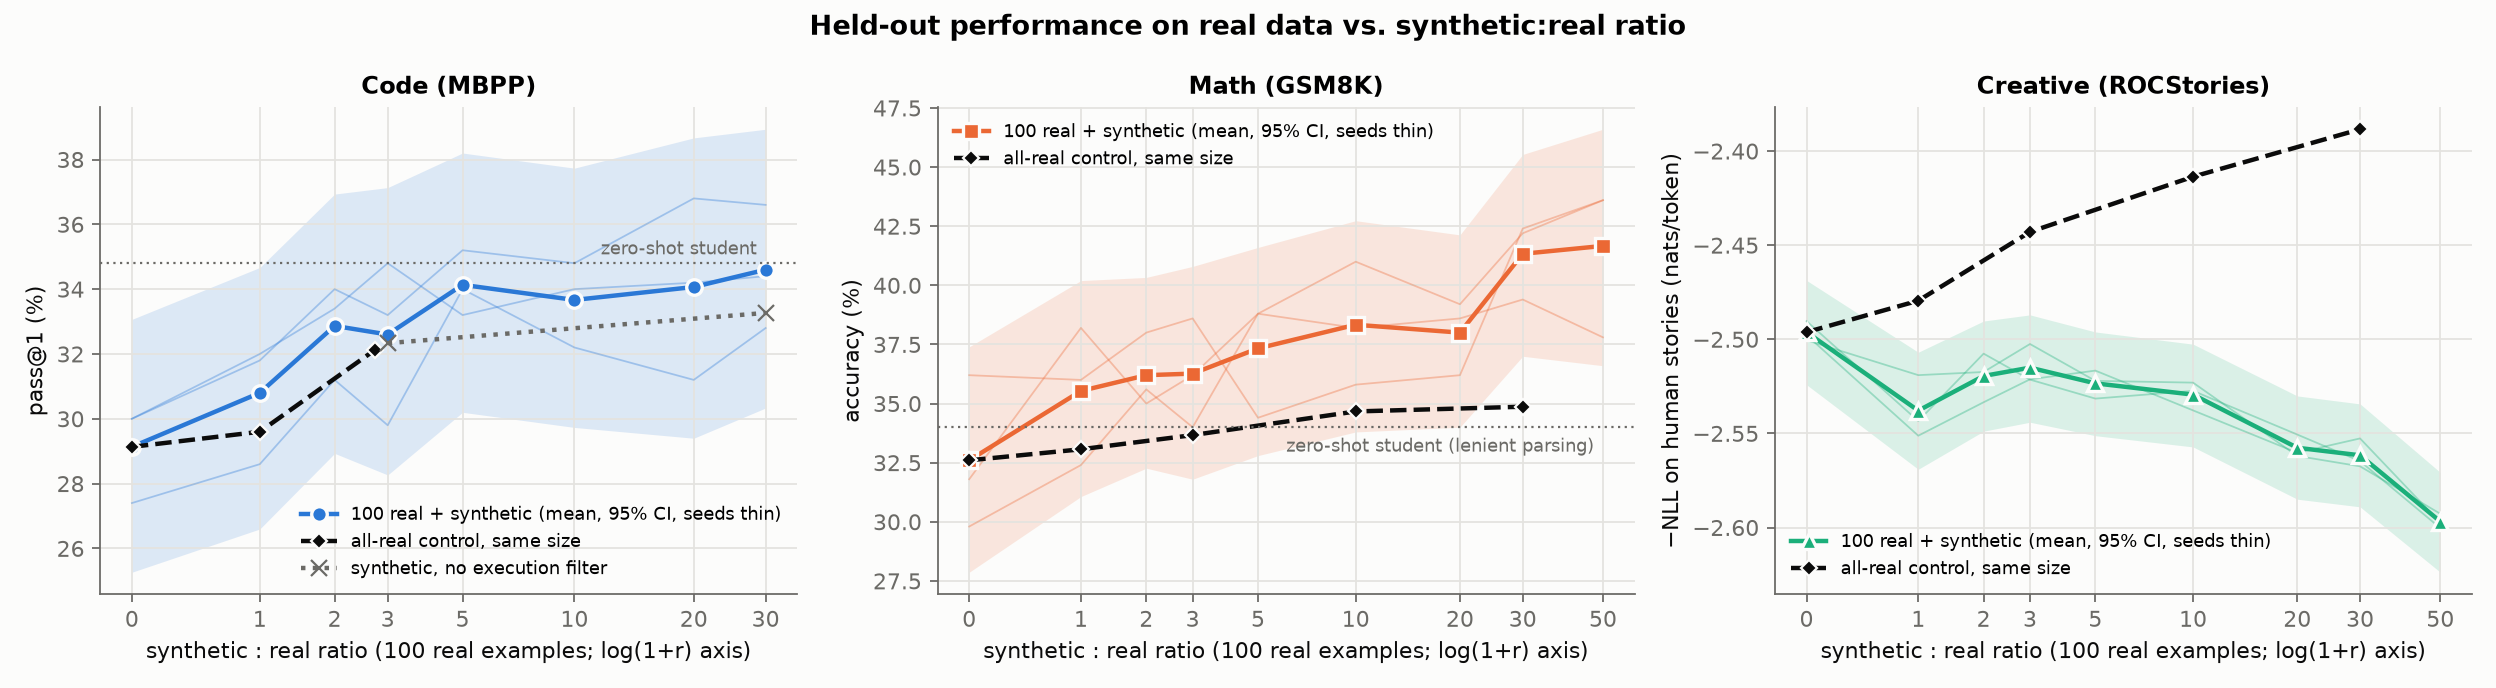
\includegraphics[width=\linewidth]{figures/dose_response.png}
    \caption{Held-out performance on real data against the synthetic-to-real ratio (mean of three seeds; shaded bands are 95\% bootstrap CIs; thin lines are seeds). Black dashed lines show the all-real control at the same training-set size. Code pass@1 rises to about \ratio{5} and then stays flat, never exceeding the zero-shot student. Math accuracy keeps rising to \ratio{50} and exceeds the all-real control. For stories, every synthetic ratio is worse than real-only training, while real data keeps helping.}
    \label{fig:dose}
\end{figure}

\begin{table}[t]
    \centering
    \caption{Task metric on real held-out data (mean of three seeds, 95\% bootstrap CI in brackets). ``Share'' is the normalized benefit $B(r)$ of \eqref{eq:benefit}; it is undefined for creative writing because no ratio beats real-only training. Best value in each ratio sweep in \textbf{bold}. The zero-shot math score uses lenient answer parsing.}
    \label{tab:main}
    \resizebox{\textwidth}{!}{%
    \begin{tabular}{@{}lcccccc@{}}
        \toprule
        & \multicolumn{2}{c}{\codetask (\mbpp)} & \multicolumn{2}{c}{\mathtask (\gsm)} & \creativetask (\roc) \\
        \cmidrule(lr){2-3} \cmidrule(lr){4-5} \cmidrule(lr){6-6}
        \textbf{Ratio} & pass@1 (\%) $\uparrow$ & share & accuracy (\%) $\uparrow$ & share & NLL on human stories $\downarrow$ \\
        \midrule
        0 (real only) & 29.1 \ci{25.3}{33.1} & 0.00 & 32.6 \ci{27.9}{37.4} & 0.00 & \textbf{2.496} \ci{2.469}{2.524} \\
        \ratio{1}  & 30.8 \ci{26.6}{34.7} & 0.30 & 35.5 \ci{31.1}{40.2} & 0.32 & 2.538 \ci{2.507}{2.569} \\
        \ratio{2}  & 32.9 \ci{28.9}{36.9} & 0.68 & 36.2 \ci{32.3}{40.3} & 0.40 & 2.520 \ci{2.490}{2.549} \\
        \ratio{3}  & 32.6 \ci{28.3}{37.1} & 0.63 & 36.3 \ci{31.8}{40.8} & 0.40 & 2.515 \ci{2.487}{2.544} \\
        \ratio{5}  & 34.1 \ci{30.2}{38.2} & 0.91 & 37.3 \ci{32.8}{41.6} & 0.52 & 2.523 \ci{2.496}{2.551} \\
        \ratio{10} & 33.7 \ci{29.7}{37.7} & 0.83 & 38.3 \ci{33.8}{42.7} & 0.63 & 2.529 \ci{2.503}{2.557} \\
        \ratio{20} & 34.1 \ci{29.4}{38.7} & 0.90 & 38.0 \ci{34.0}{42.1} & 0.60 & 2.558 \ci{2.530}{2.585} \\
        \ratio{30} & \textbf{34.6} \ci{30.3}{38.9} & 1.00 & 41.3 \ci{37.0}{45.5} & 0.96 & 2.562 \ci{2.534}{2.589} \\
        \ratio{50} & -- & -- & \textbf{41.7} \ci{36.6}{46.6} & 1.00 & 2.597 \ci{2.571}{2.624} \\
        \midrule
        All-real control, \ratio{3} size & 32.1 (at \ratio{2.74}) & & 33.7 & & 2.443 \\
        All-real control, \ratio{30} size & -- & & 34.9 & & 2.388 \\
        Zero-shot student & 34.8 & & 34.0 & & 2.908 \\
        \bottomrule
    \end{tabular}
    }
\end{table}

\para{Code saturates early.} Pass@1 rises from 29.1\% with real data only to 34.1\% at \ratio{5} and then moves by less than a point up to \ratio{30} (34.6\%).
Real-only fine-tuning makes the student \emph{worse} than zero-shot (29.1\% against 34.8\%), and the best synthetic condition only recovers to parity.
On \mbpp the benefit we measure is therefore recovery from a harmful real-only baseline, not an improvement over the untuned model.

\para{Math keeps improving.} Accuracy rises from 32.6\% to 36.3\% at \ratio{3}, 38.3\% at \ratio{10}, and 41.7\% at \ratio{50}.
The all-real control improves far less, from 32.6\% to 34.9\% at the \ratio{30} size.

\para{Stories get worse from the first synthetic example.} The NLL on human stories is lowest with no synthetic data (2.496) and rises to 2.597 at \ratio{50}.
The all-real control moves the other way, to 2.388 at the \ratio{30} size.

\subsection{Does a \ratio{3} Ratio Capture 80\% of the Benefit?}
\label{sec:h1b}

No.
The share of maximum observed gain at \ratio{3} is 0.63 for code (95\% CI 0.13--1.00) and 0.40 for math (CI 0.06--0.64).
The math interval excludes 0.8, and the share reaches 0.8 in only 0.2\% of bootstrap resamples for math and 14\% for code.
Code first reaches 80\% of its maximum at about \ratio{5}.
For math the maximum sits at the edge of the grid, so 0.40 is an upper bound on the true share.
For creative writing the share is undefined because no ratio beats real-only training.
The left panel of \figref{fig:normalised} shows the full curves.

\begin{figure}[t]
    \centering
    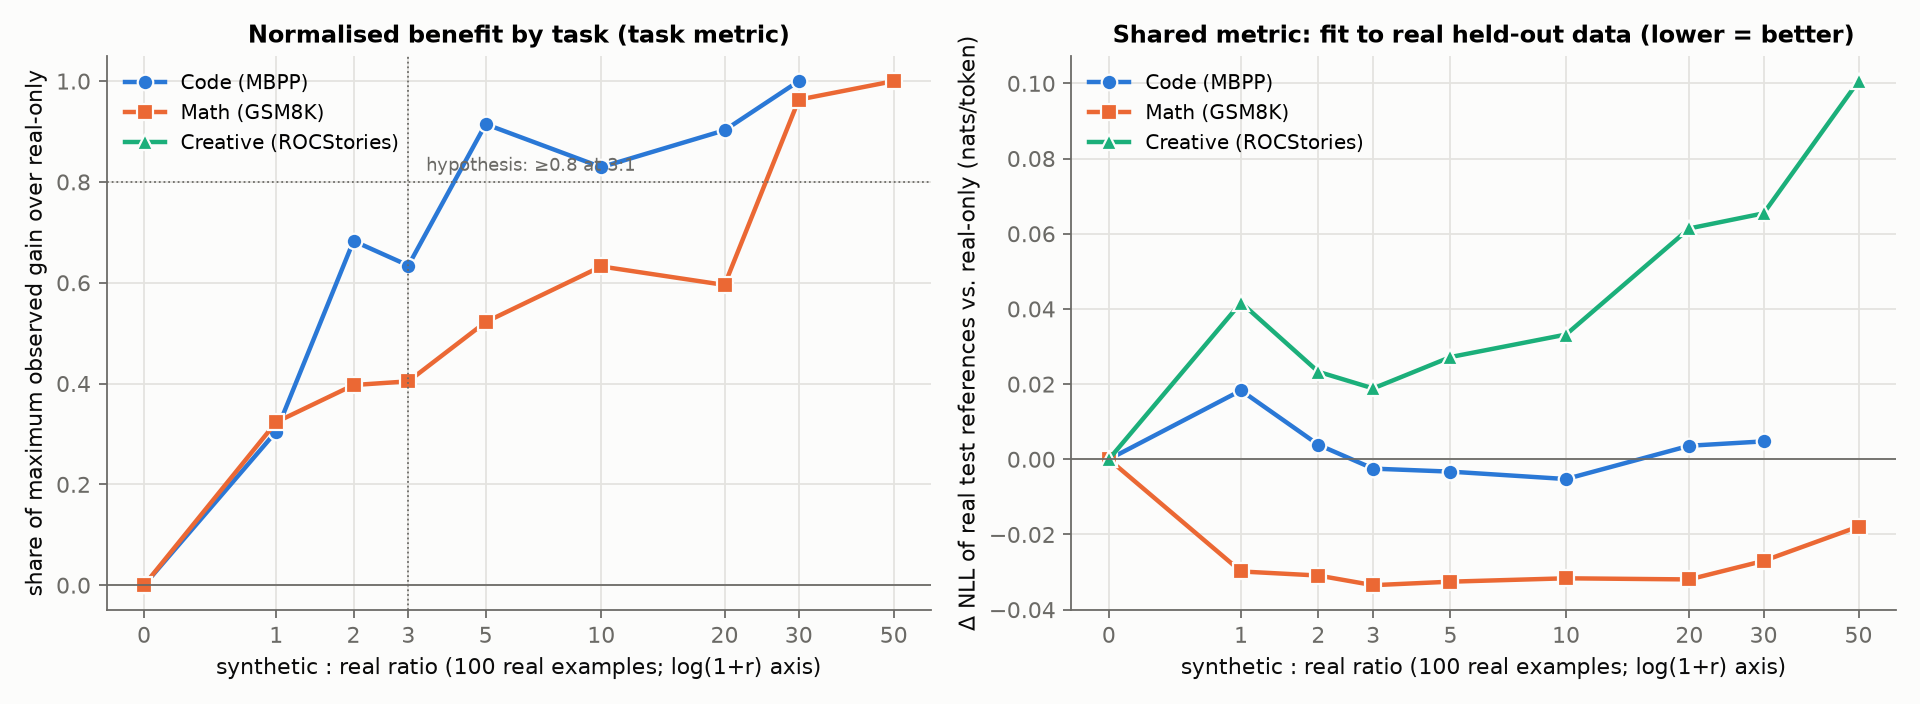
\includegraphics[width=0.95\linewidth]{figures/normalised_benefit.png}
    \caption{\figleft Share of the maximum observed gain on the task metric. The hypothesis predicts at least 0.8 at \ratio{3} (dotted lines); code reaches 0.63 and math 0.40. \figright Change in NLL on real held-out references relative to real-only training (lower is better). All three tasks degrade beyond \ratio{10}; the degradation for stories is an order of magnitude larger than for code and math.}
    \label{fig:normalised}
\end{figure}

\subsection{What Happens Beyond \ratio{10}?}
\label{sec:h2a}

\begin{table}[t]
    \centering
    \caption{Planned contrasts on the task metric: difference with 95\% CI. Code and math are in accuracy points. Creative writing is in $-$NLL (nats per token), so negative values mean a worse fit to human stories. $^{*}$ $p < 0.05$, $^{***}$ $p < 0.001$ (Holm-adjusted across tasks; unadjusted for the \ratio{50} contrast); unmarked contrasts are not significant.}
    \label{tab:contrasts}
    \begin{tabular}{@{}llll@{}}
        \toprule
        \textbf{Contrast} & \codetask (points) & \mathtask (points) & \creativetask ($-$NLL) \\
        \midrule
        \ratio{3} $-$ real-only & $+3.5^{*}$ \ci{+0.7}{+6.5} & $+3.7^{*}$ \ci{+0.6}{+6.8} & $-0.019^{*}$ \ci{-0.031}{-0.004} \\
        \ratio{10} $-$ \ratio{3} & $+1.1$ \ci{-1.9}{+3.8} & $+2.1$ \ci{-3.0}{+6.7} & $-0.014^{***}$ \ci{-0.021}{-0.007} \\
        \ratio{30} $-$ \ratio{10} & $+0.9$ \ci{-1.6}{+3.6} & $+3.0$ \ci{-1.0}{+7.3} & $-0.032^{***}$ \ci{-0.044}{-0.016} \\
        \ratio{50} $-$ \ratio{10} & -- & $+3.3$ \ci{-1.6}{+8.4} & $-0.067^{***}$ \ci{-0.074}{-0.060} \\
        \bottomrule
    \end{tabular}
\end{table}

\para{On the task metric, the answer depends on the domain.}
\Tabref{tab:contrasts} gives the planned contrasts.
For code, \ratio{30} differs from \ratio{10} by $+0.9$ points (CI $-1.6$ to $+3.6$), and the slope of pass@1 per unit of $\ln r$ for $r \geq 10$ is $+0.8$ points (CI $-1.5$ to $+3.3$): a plateau.
For math, accuracy at \ratio{30} and \ratio{50} is 3.0 and 3.3 points above \ratio{10}, and the slope is $+2.4$ points per unit of $\ln r$ (CI $-0.8$ to $+5.8$).
Neither math contrast is individually significant, so we detect no plateau but cannot exclude one.
For stories, every step is a significant loss, with a slope of $-0.040$ nats per unit of $\ln r$ (CI $-0.044$ to $-0.033$).

\para{On the shared metric, all three domains degrade.}
\Tabref{tab:nll} and the right panel of \figref{fig:normalised} show the NLL on real held-out references.
All three tasks have an interior optimum followed by degradation: the best ratio is \ratio{10} for code, \ratio{3} for math, and 0 for stories.
From \ratio{10} to \ratio{30} the NLL rises by 0.0100 nats for code, 0.0046 for math, and 0.0322 for stories, each with $p < 0.001$.
The degradation is small for code and math (at most 0.01 nats) and an order of magnitude larger for stories.
Math shows both effects at once: accuracy rises with the ratio while the fit to human-written reference solutions is best at \ratio{3} and then worsens.

\begin{table}[t]
    \centering
    \caption{Shared metric: NLL of real held-out references (nats per token; positive differences mean a worse fit). ``Best ratio'' gives the ratio with the lowest mean NLL and the share of bootstrap resamples in which it is best.}
    \label{tab:nll}
    \resizebox{0.9\textwidth}{!}{%
    \begin{tabular}{@{}llcc@{}}
        \toprule
        \textbf{Task} & \textbf{Best ratio} & \textbf{\ratio{30} $-$ \ratio{10}} & \textbf{\ratio{30} $-$ real-only} \\
        \midrule
        \codetask & \ratio{10} (85\%) & $+0.0100$ \ci{+0.0037}{+0.0183}, $p < 0.001$ & $+0.0048$ \ci{-0.0018}{+0.0119}, \ns \\
        \mathtask & \ratio{3} (61\%) & $+0.0046$ \ci{+0.0025}{+0.0069}, $p < 0.001$ & $-0.0270$ \ci{-0.0521}{-0.0067}, $p < 0.001$ \\
        \creativetask & 0 (99\%) & $+0.0322$ \ci{+0.0158}{+0.0442}, $p < 0.001$ & $+0.0654$ \ci{+0.0551}{+0.0756}, $p < 0.001$ \\
        \bottomrule
    \end{tabular}
    }
\end{table}

\subsection{Are Gains Logarithmic?}
\label{sec:h1a}

Only for math, and weakly.
\Tabref{tab:fits} compares the five curve families.
For math the logarithmic model has the lowest AICc, but it explains little variance ($R^2 = 0.28$) and the power law is within 1.6 units.
For code, bounded saturating curves fit best and the logarithmic model is 11.4 AICc units worse.
For stories the ``gain'' is negative, and a power law describes the loss best.
A linear model is the worst fit in all three domains.

\begin{table}[t]
    \centering
    \caption{Curve fits to seed-level gains: $\Delta$AICc (0 = best, in \textbf{bold}) with $R^2$ in parentheses. No single functional form wins across domains.}
    \label{tab:fits}
    \begin{tabular}{@{}lccccc@{}}
        \toprule
        \textbf{Task} & \textbf{Linear} & \textbf{Log} & \textbf{Power} & \textbf{Hyperbolic} & \textbf{Exp.\ saturation} \\
        \midrule
        \codetask & 37.7 ($-2.03$) & 11.4 (0.13) & 4.5 (0.45) & 0.6 (0.55) & \textbf{0.0} (0.56) \\
        \mathtask & 12.3 ($-0.21$) & \textbf{0.0} (0.28) & 1.6 (0.31) & 2.9 (0.27) & 4.1 (0.23) \\
        \creativetask & 14.3 (0.41) & 4.4 (0.61) & \textbf{0.0} (0.71) & 8.0 (0.60) & 9.4 (0.57) \\
        \bottomrule
    \end{tabular}
\end{table}

\subsection{Mechanism: Diversity of the Synthetic Pools}
\label{sec:diversity}

\begin{figure}[t]
    \centering
    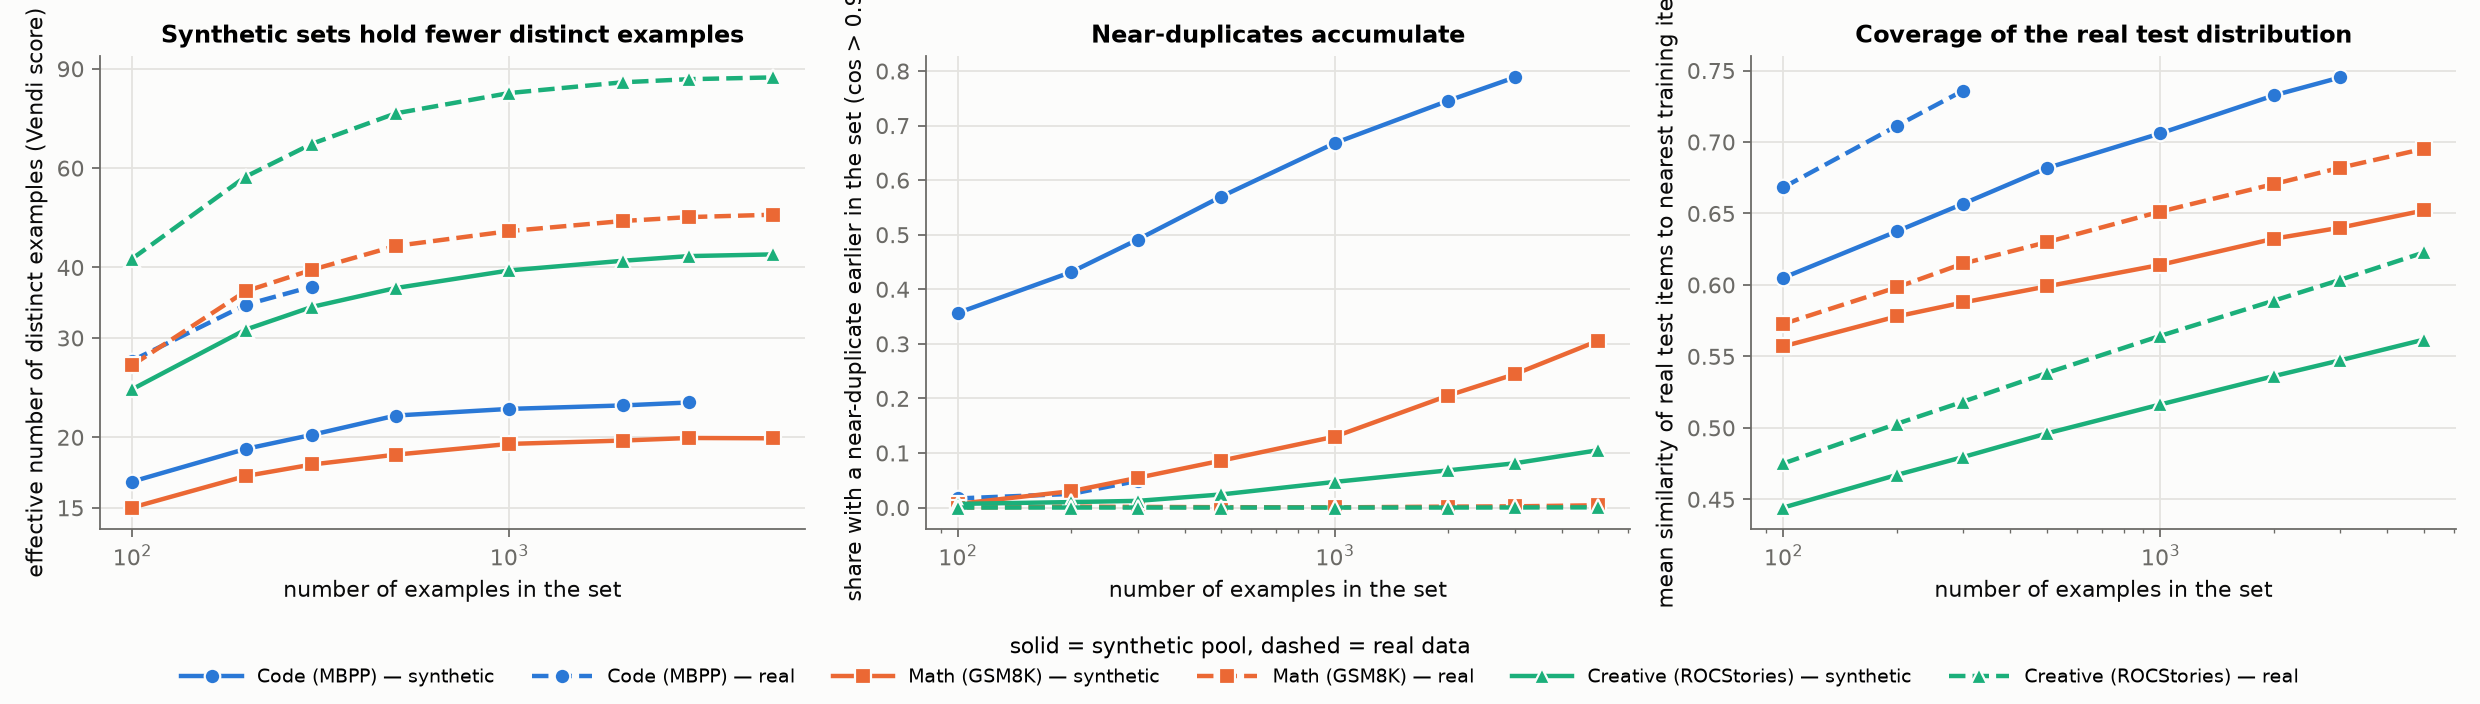
\includegraphics[width=\linewidth]{figures/pool_diversity.png}
    \caption{Diversity of synthetic pools (solid) and real data (dashed) as the set grows. \figleft The effective number of distinct examples (Vendi score) saturates for synthetic pools well below the level of real data. \figcenter Near-duplicates accumulate in synthetic pools, fastest for code, and are nearly absent in real data. \figright Synthetic data covers the real test distribution less well than real data at every size.}
    \label{fig:diversity}
\end{figure}

\begin{table}[t]
    \centering
    \caption{Diversity of synthetic pools and real data (mean over three pools). Near-duplicates have cosine similarity above 0.9 to an earlier example. ``Vendi'' is an effective number of distinct examples in embedding space. ``Coverage'' is the mean similarity of real test items to their nearest training example.}
    \label{tab:diversity}
    \resizebox{\textwidth}{!}{%
    \begin{tabular}{@{}llrccccc@{}}
        \toprule
        \textbf{Task} & \textbf{Source} & $n$ & \textbf{Exact dup.} & \textbf{Near-dup.} & \textbf{Distinct bigrams} & \textbf{Vendi} & \textbf{Coverage} \\
        \midrule
        \multirow{3}{*}{\codetask} & synthetic & 300 & 22\% & 49\% & 0.21 & 20.2 & 0.657 \\
         & synthetic & 3,000 & 44\% & 79\% & 0.08 & 23.1 & 0.745 \\
         & real & 300 & 0\% & 5\% & 0.37 & 37.0 & 0.736 \\
        \midrule
        \multirow{3}{*}{\mathtask} & synthetic & 300 & 0\% & 5\% & 0.43 & 17.9 & 0.588 \\
         & synthetic & 5,000 & 0.2\% & 31\% & 0.15 & 19.9 & 0.652 \\
         & real & 5,000 & 0\% & 0.4\% & 0.39 & 49.6 & 0.695 \\
        \midrule
        \multirow{3}{*}{\creativetask} & synthetic & 300 & 0\% & 1\% & 0.62 & 34.1 & 0.480 \\
         & synthetic & 5,000 & 0\% & 11\% & 0.30 & 42.2 & 0.562 \\
         & real & 5,000 & 0\% & 0.0\% & 0.42 & 86.9 & 0.623 \\
        \bottomrule
    \end{tabular}
    }
\end{table}

{\bf Does the generator collapse onto a few modes?} Yes.
\Tabref{tab:diversity} and \figref{fig:diversity} compare synthetic pools with real data.
In a 3,000-example code pool, 44\% of task descriptions are exact duplicates and 79\% have a near-duplicate, against 0\% and 5\% for 300 real \mbpp problems.
In the seed-0 pools, \texttt{factorial} is the function in 523 of 3,626 usable code examples (14\%) and \texttt{fibonacci} in 197; 1,232 of 5,174 math problems (24\%) begin with ``Sarah''; and story titles concentrate on variants of ``The Book Swap'' (257), ``The Lost Key'' (256), and ``Birthday Surprise'' (159).

Growing a pool adds little that is new.
Going from 300 to 3,000--5,000 synthetic examples raises the Vendi score by only 14\% for code, 11\% for math, and 24\% for stories.
At 5,000 examples the Vendi score of synthetic data is 40\% of that of real data for math (19.9 against 49.6) and 49\% for stories (42.2 against 86.9).
Synthetic data needs roughly 5--10 times as many examples as real data to reach the same coverage of the real test set: 5,000 synthetic math problems reach the coverage of 1,000 real ones (0.652 against 0.651), and 3,000 synthetic code tasks reach that of 300 real ones (0.745 against 0.736).

The code pools are the most collapsed, and code is the domain where accuracy saturates earliest.
This is consistent with H2b: beyond about \ratio{5} a larger code pool adds almost no new problems.
The evidence is correlational, because we do not vary diversity at fixed pool size.

\subsection{What the Student Writes}
\label{sec:creative}

\begin{figure}[t]
    \centering
    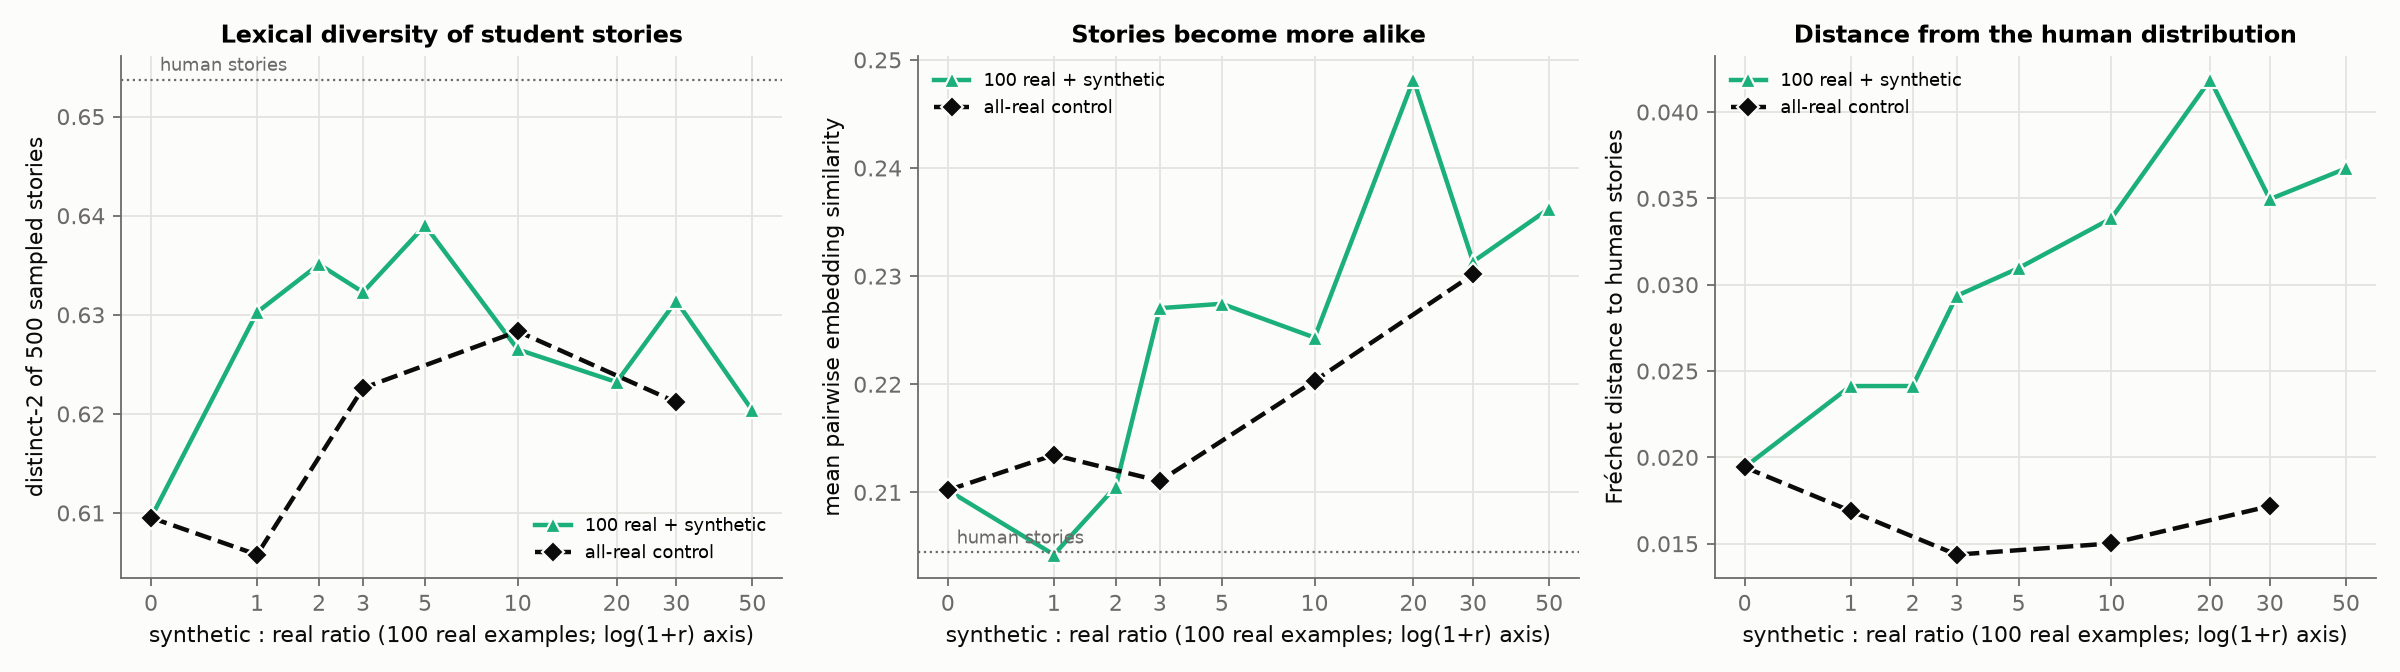
\includegraphics[width=\linewidth]{figures/creative_generation.png}
    \caption{Properties of 500 sampled student stories per model. \figleft Lexical diversity (distinct-2) does not fall with the synthetic ratio. \figcenter Stories become more similar to each other in embedding space. \figright The Fr\'echet distance to human stories roughly doubles with synthetic data, while the all-real control stays near the noise floor of 0.013.}
    \label{fig:creative}
\end{figure}

\begin{table}[t]
    \centering
    \caption{Properties of 500 sampled student stories (mean over seeds). The Fr\'echet distance reported for human stories is the noise floor of the estimate. Values closest to human stories among trained students in \textbf{bold}.}
    \label{tab:creative}
    \resizebox{0.95\textwidth}{!}{%
    \begin{tabular}{@{}lcccc@{}}
        \toprule
        \textbf{Condition} & \textbf{Distinct-2} & \textbf{Pairwise similarity} & \textbf{Fr\'echet distance} $\downarrow$ & \textbf{Five sentences} \\
        \midrule
        Human stories & 0.654 & 0.204 & 0.013 & 99.8\% \\
        \midrule
        Real only ($r = 0$) & 0.610 & \textbf{0.210} & 0.019 & 69\% \\
        Synthetic \ratio{3} & \textbf{0.632} & 0.227 & 0.029 & 77\% \\
        Synthetic \ratio{30} & 0.631 & 0.231 & 0.035 & 70\% \\
        Synthetic \ratio{50} & 0.620 & 0.236 & 0.037 & 77\% \\
        All-real control, \ratio{30} size & 0.621 & 0.230 & \textbf{0.017} & \textbf{98\%} \\
        \bottomrule
    \end{tabular}
    }
\end{table}

\Tabref{tab:creative} and \figref{fig:creative} describe the stories that students sample.
The Fr\'echet distance to human stories rises from 0.019 with real data only to 0.035 at \ratio{30} and 0.037 at \ratio{50}; the all-real control at the \ratio{30} size stays at 0.017.
Only the all-real control learns the format: 98\% of its stories have exactly five sentences, against 69--77\% for the other conditions.

\para{Lexical diversity does not collapse.} Distinct-2 of student stories is not lower with synthetic data (0.62--0.64 against 0.61 for real-only).
The homogenization shows up in content: mean pairwise embedding similarity rises from 0.210 to 0.236 at \ratio{50}, and stories converge on the teacher's preferred names and scenarios.
The all-real control at the \ratio{30} size also reaches a pairwise similarity of 0.230, so this statistic alone does not separate synthetic from real training; the Fr\'echet distance and the inherited modes below do.

\para{Students inherit the teacher's modes.} We count occurrences of the name ``Sarah'' in 500 stories (seed 0).
Human test stories contain 8 and the first 500 synthetic stories contain 375.
The student contains 11 after real-only training, 13 after the all-real control, and 171 after \ratio{30} training, a 15-fold increase.
For the title ``Kitchen Table'', the all-real student writes: \emph{``Jane was creating a remodel for her home. She wanted to make the kitchen. She did a great job with the room. She showed her neighbors. They said the kitchen looked pretty.''}
The \ratio{30} student writes: \emph{``At the kitchen table, Sarah decided to bake a cake. She placed all her ingredients on a rimmed baking sheet. Unexpectedly, the hot baking sheets melted away. Relieved, she let the cake cool, then took a photo to show her husband.''}

\subsection{Synthetic Against Real Data at Equal Size}
\label{sec:synth_vs_real}

The all-real control separates the source of the data from its amount (\tabref{tab:synth_real} in the appendix).
For stories, real data wins at every size, and the gap grows from 0.058 nats at the \ratio{1} size to 0.173 at the \ratio{30} size.
For math, the synthetic mix wins on accuracy, and the gap also grows: $+3.7$ points at the \ratio{10} size (CI $+0.4$ to $+7.0$, $p = 0.030$) and $+6.5$ points at the \ratio{30} size (CI $+2.3$ to $+11.0$, $p = 0.002$).
This holds even though the all-real model fits the real references far better (NLL 0.637 against 0.682).
For code the control only extends to \ratio{2.74}, where real data scores 32.1\% against 32.6\% for the synthetic mix at \ratio{3}.

\subsection{Error Analysis and Ablation}
\label{sec:errors}

\para{Code.} Wrong answers dominate failures: 52--55\% of test items raise an assertion error at every ratio. From real-only to \ratio{30}, synthetic data reduces other runtime errors from 4.6\% to 2.5\% of items and wrong answers from 55.0\% to 51.9\%, while syntax errors stay near 1\%. The zero-shot student makes more syntax errors (5.0\%) but fewer wrong answers (48.0\%).

\para{Math.} Almost all failures are wrong final answers, which fall from 66\% of items with real data only to 55\% at \ratio{50}. Format failures (no answer line) stay between 1\% and 6\%.

\para{Execution filter.} Without the execution filter on the code pool, pass@1 is 32.3\% at \ratio{3} and 33.3\% at \ratio{30}, against 32.6\% and 34.6\% with it. The per-seed differences at \ratio{30} go both ways ($+0.2$, $-1.4$, $+5.2$ points), so the ablation is inconclusive.

\section{Discussion}
\label{sec:discussion}

\begin{table}[t]
    \centering
    \caption{Verdict for each part of the hypothesis.}
    \label{tab:verdict}
    \renewcommand{\arraystretch}{1.2}
    \resizebox{\textwidth}{!}{%
    \begin{tabular}{@{}llp{9.2cm}@{}}
        \toprule
        \textbf{Claim} & \textbf{Verdict} & \textbf{Evidence} \\
        \midrule
        H1a: gains are logarithmic & Partly (math only) & Log is the best model for math but explains little variance ($R^2 = 0.28$). Code follows a bounded saturating curve; creative ``gains'' are negative. \\
        H1b: 80\% of benefit at \ratio{3} & Not supported & Code 63\% (CI 13--100\%), math 40\% (CI 6--64\%), undefined for creative writing. \\
        H2a: plateau or degradation beyond \ratio{10} & Depends on domain and metric & Code accuracy plateaus; math accuracy shows no plateau up to \ratio{50}; creative fit degrades. NLL on real references degrades in all three. \\
        H2b: mode collapse is the mechanism & Consistent, not proven & Pool diversity saturates and students inherit teacher modes, but we do not manipulate diversity. \\
        H3: code most resilient, creative earliest & Half supported & Creative writing degrades from the first synthetic example. Code is stable, but math tolerates and benefits from the highest ratios. \\
        \bottomrule
    \end{tabular}
    }
\end{table}

\Tabref{tab:verdict} summarizes the verdicts.
We now interpret the pattern and state what the study cannot show.

\para{Two effects pull in opposite directions.}
Synthetic data transfers the teacher's \emph{skill}, which helps where an answer is right or wrong, and the teacher's \emph{distribution}, which hurts where the target is the human distribution.
Math shows both at once: the student becomes a better solver while it becomes a worse imitator of the reference style of \gsm.
Stories have no skill component in our metrics, so only the distribution shift is visible.
This view explains why the task metric and the shared metric disagree beyond \ratio{10}, and why no single ceiling exists.

\para{Why does synthetic math data beat real data?}
At the \ratio{30} size the synthetic mix is 6.5 points more accurate than 3,100 real \gsm examples.
We did not expect this.
A plausible explanation, which we did not test, is that the teacher's worked solutions are more uniform and explicit than human-written ones, and that a 0.5B model learns from them more easily.
We also did not verify the correctness of the teacher's math solutions.

\para{Why does code saturate early?}
The code pools are the most collapsed, with 79\% near-duplicates at 3,000 examples, so ratios beyond about \ratio{5} add almost no new problems.
The student keeps re-reading \texttt{factorial}.
The execution filter may contribute by favoring easy problems the teacher can solve, but our ablation cannot settle this.

\para{Small doses can be the worst doses.}
On the shared metric, \ratio{1} is the worst ratio for code and is worse than every ratio from \ratio{2} to \ratio{10} for stories.
One reading, which we did not test, is that a small amount of synthetic data shifts the distribution without yet adding much skill.

\para{Diversity metrics can miss homogenization.}
Distinct-2 of student stories does not fall with the synthetic ratio, while the Fr\'echet distance to human stories roughly doubles and one teacher-preferred name becomes 15 times more frequent.
Studies that track only $n$-gram diversity would miss this.

\para{Practical implications.}
For verifiable skills such as code and arithmetic reasoning, extra synthetic data did not hurt task accuracy up to \ratio{30}--\ratio{50} in our setting, but most of the code benefit arrived by about \ratio{5}.
For open-ended generation, where the goal is to match a human distribution, synthetic data from a single generator hurt at every ratio we tested, and 100 more real examples were worth more than 5,000 synthetic ones.

\subsection{Limitations}
\label{sec:limitations}

\para{Statistical power.} Three seeds and 500 test items give 95\% CIs of about $\pm 4$ points on accuracy. Differences of under about 4 points between adjacent ratios are within noise. Only the \ratio{3}-against-0 and peak-against-0 contrasts are significant for code and math, so ``plateau'' for code and ``still rising'' for math are statements our data cannot sharply distinguish. A seed-level bootstrap with three seeds is coarse. The NLL-based results are much tighter.

\para{The share statistic.} $B(3)$ uses the maximum over a noisy grid, which biases the share at \ratio{3} downward. The location of the code maximum is itself uncertain: \ratio{30} is the best ratio in only 39\% of bootstrap resamples. For math the maximum is at the edge of the grid.

\para{One configuration.} We use one teacher (3B), one student (0.5B, LoRA rank 32), one real-set size (100), and one generation recipe (3-shot, $T = 1$, no de-duplication, no diversity prompting). A stronger teacher, attribute-controlled prompting~\citep{yu2023attributed}, or de-duplication would likely move the curves.

\para{Training budget.} We train for at most two epochs with early stopping, so larger ratios receive more gradient steps. We did not match compute across ratios.

\para{Code is not directly comparable to the other domains.} Its pool is execution-filtered, its grid stops at \ratio{30}, and its real-data control stops at \ratio{2.74} because \mbpp is small.

\para{Creative quality.} We measure fit to human text and distributional distance. We collected no human or model-judge ratings of story quality; synthetic-trained stories may read as more polished while being less human-like.

\para{Contamination.} \mbpp, \gsm, and \roc are probably in the pre-training data of both models. This affects absolute levels more than the comparison between ratios.

\para{Zero-shot math baseline.} The 256-token generation cap depresses the zero-shot math score; a pilot with 320 tokens on all 1,319 test items gave 41.8\%.

\para{Mechanism.} The link between mode collapse and the dose--response curves is correlational. No experiment varied pool diversity while holding size fixed.

\section{Conclusion}
\label{sec:conclusion}

We measured how held-out performance on real data changes with the synthetic-to-real ratio across code, math, and story writing under one protocol.
Synthetic data from a stronger model gave diminishing but not uniformly capped returns: code accuracy saturated near \ratio{5}, math accuracy kept improving to \ratio{50}, and fit to human stories got worse from the first synthetic example.
The ``80\% at \ratio{3}'' rule did not hold, and ``beyond \ratio{10} hurts'' held for fidelity to real data in all three domains but for the task metric only in creative writing.
Generator mode collapse is large and measurable after a single round of generation, and students inherit it.

The main takeaway is that the right amount of synthetic data depends on what the student should learn: a skill that can be checked tolerates high ratios, while a human distribution that must be matched does not.

Several follow-ups would sharpen these conclusions.
A causal test with de-duplicated or diversity-prompted pools at fixed size would show whether mode collapse causes the code plateau.
More seeds and full test sets at ratios from 5 to 100 would locate where, or whether, math accuracy turns over.
Stronger teachers, other real-set sizes, compute-matched training, and human ratings of stories would test how far the pattern generalizes.
One question remains open: why did synthetic math data beat the same amount of real data on accuracy?


\bibliography{references}

\appendix
\section{Implementation Details}
\label{sec:app_details}

\para{Student.} LoRA rank 32, $\alpha = 64$, applied to all attention and MLP projections (17.6M trainable parameters); AdamW with learning rate $10^{-4}$ and weight decay 0.01; batch size 8; 10\% warm-up followed by cosine decay; training length of $\max$(2 epochs, 100 steps); maximum sequence length 448; six validation checks per run with the best checkpoint selected by loss on the real validation set.
Generation uses at most 256 new tokens for code and math and 96 for stories.

\para{Teacher.} \teacher in bf16, temperature 1.0, top-$p$ 0.95, at most 512 new tokens. We treat outputs that do not parse, or that contain CJK characters (the teacher occasionally code-switches at $T = 1$), as format violations and discard them.

\para{Synthetic pools.} \Tabref{tab:pools} gives the yield of each pool.

\begin{table}[h]
    \centering
    \caption{Synthetic pools per seed.}
    \label{tab:pools}
    \resizebox{\textwidth}{!}{%
    \begin{tabular}{@{}lccl@{}}
        \toprule
        \textbf{Task} & \textbf{Requests} & \textbf{Usable} & \textbf{Filter} \\
        \midrule
        \codetask & 7,000 & 3,527--3,830 (51--55\%) & parses and passes the teacher's own three assertions \\
        \mathtask & 5,200 & 5,166--5,174 (99\%) & parses with a numeric final answer \\
        \creativetask & 5,200 & 5,197--5,199 ($\sim$100\%) & parses \\
        \bottomrule
    \end{tabular}
    }
\end{table}

\para{Data splits.} Only the train split of \roc (2018 release) has titles, so we carve its validation and test sets from that split.
For \gsm, accuracy uses the first 500 of the 1,319 test items and NLL uses all of them.

\para{Compute.} We used four RTX A6000 GPUs (48\,GB) shared with other jobs, with typically 5--20\,GB free per card. Student runs peaked at 9.0\,GB. The 117 runs took 9.2 worker-hours (about 2 hours of wall-clock time with up to five workers). Pool generation took about 52,000 teacher requests and 35 minutes. We used no API models.

\para{Software.} vLLM 0.30, PyTorch 2.13, transformers 5.19, PEFT 0.21, sentence-transformers, and SciPy.

\section{Deviations from the Pre-Specified Plan}
\label{sec:app_deviations}

We wrote the analysis plan before running experiments.
We made the following changes before producing any fine-tuned result reported here; pilot runs made under earlier settings were deleted and re-run.
\begin{itemize}[leftmargin=*,itemsep=0pt,topsep=0pt]
    \item {\bf Teacher: 7B $\rightarrow$ 3B.} The 7B model could not generate at useful throughput in the GPU memory available on shared cards.
    \item {\bf Student: full fine-tuning $\rightarrow$ LoRA,} with the epoch cap lowered from 3 to 2 after pilots showed validation loss reaching its minimum after about one epoch. Memory constraints forced this change.
    \item {\bf Ratio grid:} $\{0, 0.5, 1, 2, 3, 5, 10, 20, 50\} \rightarrow \{0, 1, 2, 3, 5, 10, 20, 30\}$, with \ratio{50} for math and creative writing only. The 3B teacher's code passes its own tests only about 51\% of the time, so the code pools cannot support \ratio{50}. The planned \ratio{50}-against-\ratio{10} contrast therefore became \ratio{30} against \ratio{10} for code.
    \item {\bf Real-data control sizes} matched to ratios $\{1, 3, 10, 30\}$ for math and creative writing and $\{1, 2.74\}$ for code.
    \item {\bf Generation-based evaluation on 500 test items} per task with capped output length.
    \item {\bf Ablations:} the unfiltered-code ablation was reduced to ratios 3 and 30, and we did not collect model-judge ratings of story quality.
\end{itemize}

\section{Additional Results}
\label{sec:app_results}

\begin{figure}[h]
    \centering
    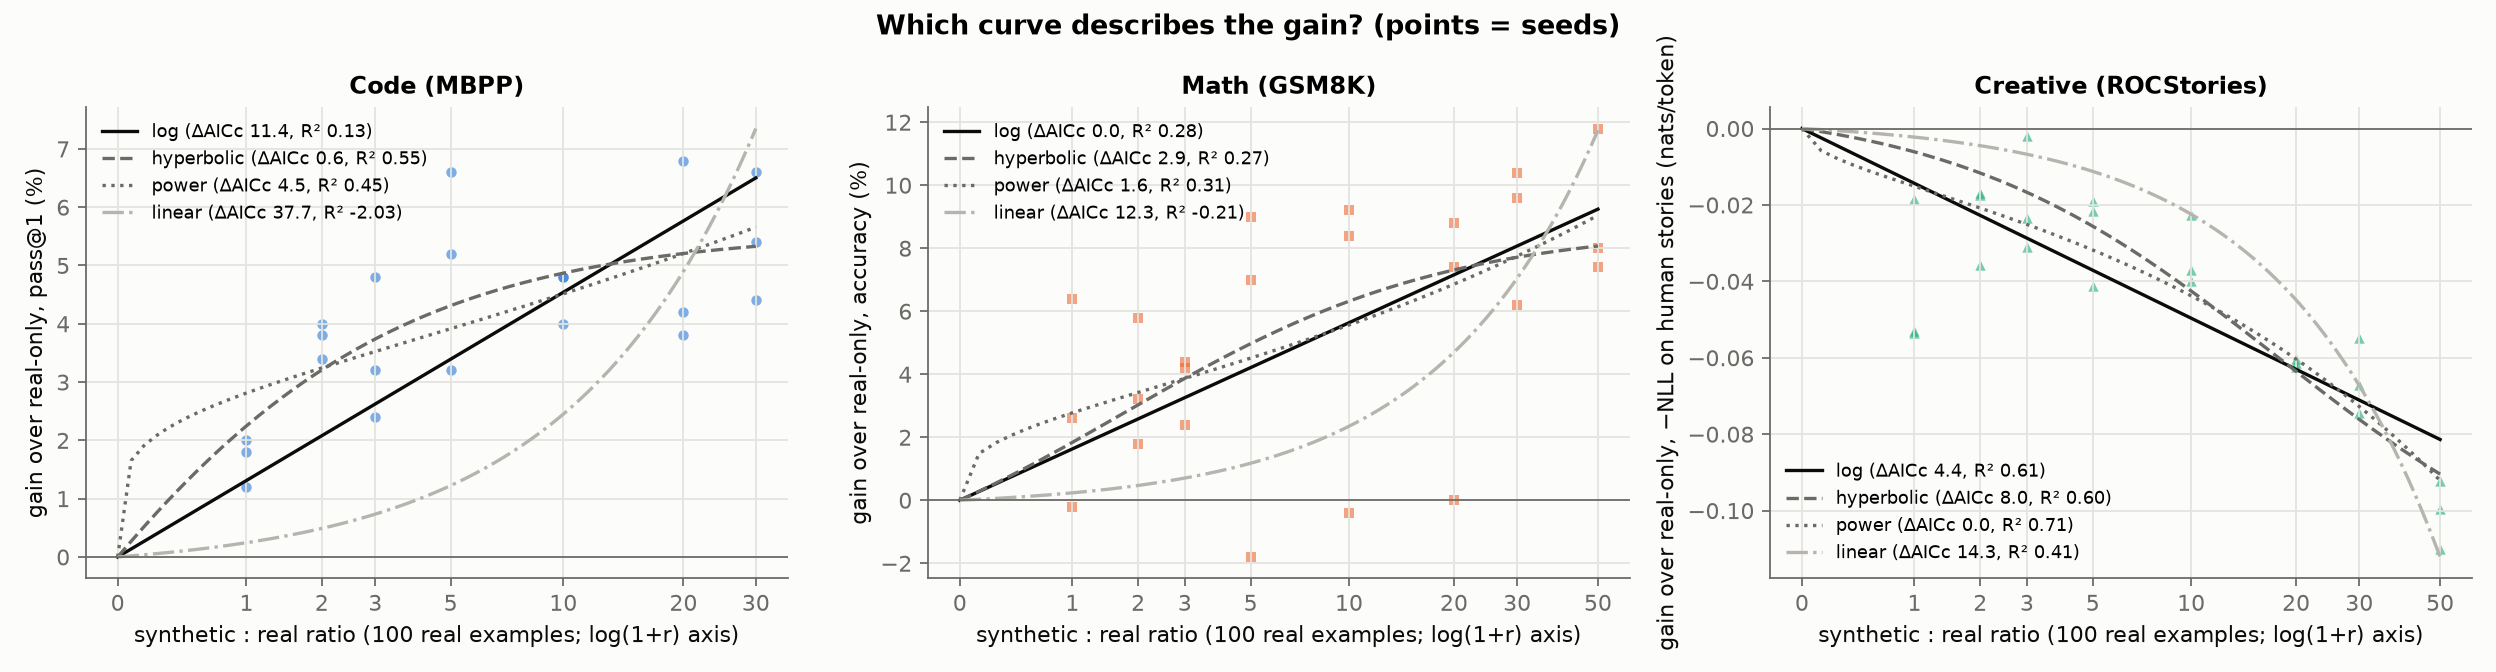
\includegraphics[width=\linewidth]{figures/curve_fits.png}
    \caption{Curve fits to seed-level gains over real-only training (points are seeds). The exponential-saturation curve is omitted because it nearly coincides with the hyperbolic one. The spread of seeds around every curve is large for code and math, which is why the fits explain little variance.}
    \label{fig:fits}
\end{figure}

\begin{table}[h]
    \centering
    \caption{Synthetic mix minus all-real control at the same training-set size, on the task metric (95\% CI; unadjusted two-sided $p$). Code and math are in accuracy points; creative writing is in $-$NLL, so negative values favor real data.}
    \label{tab:synth_real}
    \begin{tabular}{@{}llcc@{}}
        \toprule
        \textbf{Task} & \textbf{Size} & \textbf{Difference} & $p$ \\
        \midrule
        \codetask & \ratio{1} & $+1.2$ \ci{-2.1}{+4.4} & 0.424 \\
        \midrule
        \mathtask & \ratio{1} & $+2.5$ \ci{-0.8}{+5.9} & 0.138 \\
        \mathtask & \ratio{3} & $+2.6$ \ci{-0.4}{+5.4} & 0.088 \\
        \mathtask & \ratio{10} & $+3.7$ \ci{+0.4}{+7.0} & 0.030 \\
        \mathtask & \ratio{30} & $+6.5$ \ci{+2.3}{+11.0} & 0.002 \\
        \midrule
        \creativetask & \ratio{1} & $-0.058$ \ci{-0.076}{-0.037} & $<0.001$ \\
        \creativetask & \ratio{3} & $-0.072$ \ci{-0.082}{-0.060} & $<0.001$ \\
        \creativetask & \ratio{10} & $-0.116$ \ci{-0.126}{-0.108} & $<0.001$ \\
        \creativetask & \ratio{30} & $-0.173$ \ci{-0.184}{-0.161} & $<0.001$ \\
        \bottomrule
    \end{tabular}
\end{table}

\begin{table}[h]
    \centering
    \caption{Task metric per seed. Code is pass@1 (\%), math is accuracy (\%), and creative writing is NLL on human stories (nats per token).}
    \label{tab:perseed}
    \resizebox{\textwidth}{!}{%
    \begin{tabular}{@{}llccccccccc@{}}
        \toprule
        \textbf{Task} & \textbf{Seed} & 0 & \ratio{1} & \ratio{2} & \ratio{3} & \ratio{5} & \ratio{10} & \ratio{20} & \ratio{30} & \ratio{50} \\
        \midrule
        \multirow{3}{*}{\codetask} & 0 & 30.0 & 32.0 & 33.4 & 34.8 & 33.2 & 34.0 & 34.2 & 34.4 & -- \\
         & 1 & 27.4 & 28.6 & 31.2 & 29.8 & 34.0 & 32.2 & 31.2 & 32.8 & -- \\
         & 2 & 30.0 & 31.8 & 34.0 & 33.2 & 35.2 & 34.8 & 36.8 & 36.6 & -- \\
        \midrule
        \multirow{3}{*}{\mathtask} & 0 & 31.8 & 38.2 & 35.0 & 36.2 & 38.8 & 41.0 & 39.2 & 42.2 & 43.6 \\
         & 1 & 36.2 & 36.0 & 38.0 & 38.6 & 34.4 & 35.8 & 36.2 & 42.4 & 43.6 \\
         & 2 & 29.8 & 32.4 & 35.6 & 34.0 & 38.8 & 38.2 & 38.6 & 39.4 & 37.8 \\
        \midrule
        \multirow{3}{*}{\creativetask} & 0 & 2.50 & 2.55 & 2.53 & 2.52 & 2.52 & 2.54 & 2.56 & 2.55 & 2.60 \\
         & 1 & 2.50 & 2.52 & 2.52 & 2.50 & 2.52 & 2.52 & 2.56 & 2.57 & 2.59 \\
         & 2 & 2.49 & 2.54 & 2.51 & 2.52 & 2.53 & 2.53 & 2.55 & 2.56 & 2.60 \\
        \bottomrule
    \end{tabular}
    }
\end{table}

\begin{table}[h]
    \centering
    \caption{Error breakdown on \mbpp (share of test items, pooled over seeds).}
    \label{tab:errors_code}
    \resizebox{\textwidth}{!}{%
    \begin{tabular}{@{}lccccccc@{}}
        \toprule
        \textbf{Condition} & \textbf{Pass} & \textbf{Assertion} & \textbf{TypeError} & \textbf{NameError} & \textbf{SyntaxError} & \textbf{Other runtime} & \textbf{Timeout} \\
        \midrule
        Real only & 29.1\% & 55.0\% & 8.3\% & 1.8\% & 1.0\% & 4.6\% & 0.2\% \\
        \ratio{1} & 30.8\% & 53.0\% & 7.8\% & 2.2\% & 1.3\% & 4.3\% & 0.5\% \\
        \ratio{2} & 32.9\% & 54.3\% & 7.0\% & 1.6\% & 1.1\% & 2.8\% & 0.4\% \\
        \ratio{3} & 32.6\% & 54.6\% & 6.5\% & 1.7\% & 1.2\% & 2.8\% & 0.6\% \\
        \ratio{5} & 34.1\% & 52.2\% & 7.3\% & 2.0\% & 0.8\% & 3.1\% & 0.4\% \\
        \ratio{10} & 33.7\% & 53.6\% & 6.9\% & 1.0\% & 1.5\% & 3.1\% & 0.2\% \\
        \ratio{20} & 34.1\% & 52.9\% & 7.4\% & 1.3\% & 1.3\% & 2.7\% & 0.4\% \\
        \ratio{30} & 34.6\% & 51.9\% & 7.9\% & 1.7\% & 1.1\% & 2.5\% & 0.3\% \\
        \midrule
        Zero-shot student & 34.8\% & 48.0\% & 7.2\% & 2.0\% & 5.0\% & 2.8\% & 0.2\% \\
        \bottomrule
    \end{tabular}
    }
\end{table}

\begin{table}[h]
    \centering
    \caption{Error breakdown on \gsm (share of test items, pooled over seeds).}
    \label{tab:errors_math}
    \begin{tabular}{@{}lccc@{}}
        \toprule
        \textbf{Condition} & \textbf{Correct} & \textbf{Wrong answer} & \textbf{No answer line} \\
        \midrule
        Real only & 32.6\% & 66.2\% & 1.2\% \\
        \ratio{1} & 35.5\% & 62.4\% & 2.1\% \\
        \ratio{2} & 36.2\% & 58.3\% & 5.5\% \\
        \ratio{3} & 36.3\% & 60.3\% & 3.4\% \\
        \ratio{5} & 37.3\% & 59.5\% & 3.1\% \\
        \ratio{10} & 38.3\% & 57.9\% & 3.7\% \\
        \ratio{20} & 38.0\% & 58.3\% & 3.7\% \\
        \ratio{30} & 41.3\% & 56.2\% & 2.5\% \\
        \ratio{50} & 41.7\% & 54.7\% & 3.7\% \\
        \bottomrule
    \end{tabular}
\end{table}


\end{document}
